\documentclass{article}
\usepackage{amsmath}
\usepackage{amsfonts} 
\usepackage{physics} 
\usepackage{rotating}
\usepackage{enumitem}
\setlength{\headheight}{15pt}
\usepackage[italian]{varioref}
\usepackage{hyperref}
\usepackage{steinmetz}
\hypersetup{colorlinks=true, linkcolor=magenta, citecolor=green, urlcolor=blue} 
\usepackage{mathtools}
\hypersetup{linktoc=page}
\usepackage{extramarks}
\usepackage{amssymb}
\usepackage{fancyhdr}
\usepackage{float}
\usepackage{geometry}
 \geometry{
 a4paper,
 total={190mm,257mm},
 left=15mm,
 right=15mm,
 top=20mm,
 }
\usepackage{graphicx}
\usepackage{cancel}
\graphicspath{ {./images/} }
\usepackage{amsthm}
\usepackage{etoolbox}
\BeforeBeginEnvironment{minipage}{\medskip}
\AfterEndEnvironment{minipage}{\medskip}
\usepackage{tocloft}
\usepackage{indentfirst}
\usepackage{afterpage}
\numberwithin{equation}{section}
\newcommand\blankpage{%
    \null
    \thispagestyle{empty}%
    \addtocounter{page}{-1}%
    \newpage}
\newcommand\blankpagewnumber{%
    \null
    \newpage}
\newcommand{\T}{\mathcal{T}}
\newcommand{\U}{\mathcal{U}}
\renewcommand{\L}{\mathcal{L}}
\usepackage{blkarray, bigstrut}
\usepackage[T1]{fontenc}

\begin{document}
\afterpage{\blankpage}
\begin{titlepage}
\begin{center}
\huge Master's degree in Computer Engineering for Robotics and Smart Industry
\end{center}
\vspace*{\fill}
\begin{center}
\textbf{\Huge Advanced control systems}
\end{center}
\begin{center}
Report on the assignments given during the 2022/2023 a.y.
\end{center}
\vspace*{\fill}
\begin{center}
\begin{minipage}{0.4\textwidth}
\begin{flushleft}
Author: Lorenzo Busellato, VR472249\\
email: lorenzo.busellato\_02@studenti.univr.it
\end{flushleft}
\end{minipage}
\begin{minipage}{0.5\textwidth}
\begin{flushright}

\includegraphics[keepaspectratio,width=0.6\textwidth]{logo}
\end{flushright}
\end{minipage}

\end{center}
\vspace{1cm}
\end{titlepage}


\afterpage{\blankpage}
\thispagestyle{empty}
\setcounter{page}{0}
\pagenumbering{gobble}
\renewcommand{\cftsecleader}{\cftdotfill{\cftdotsep}}
\setcounter{tocdepth}{2}
\tableofcontents
\clearpage

\fancyhead[R]{}
\fancyhead[L]{}
\pagestyle{fancy}
\pagenumbering{arabic}

\section{Assignment 1}

\begin{figure}[h]
\centering
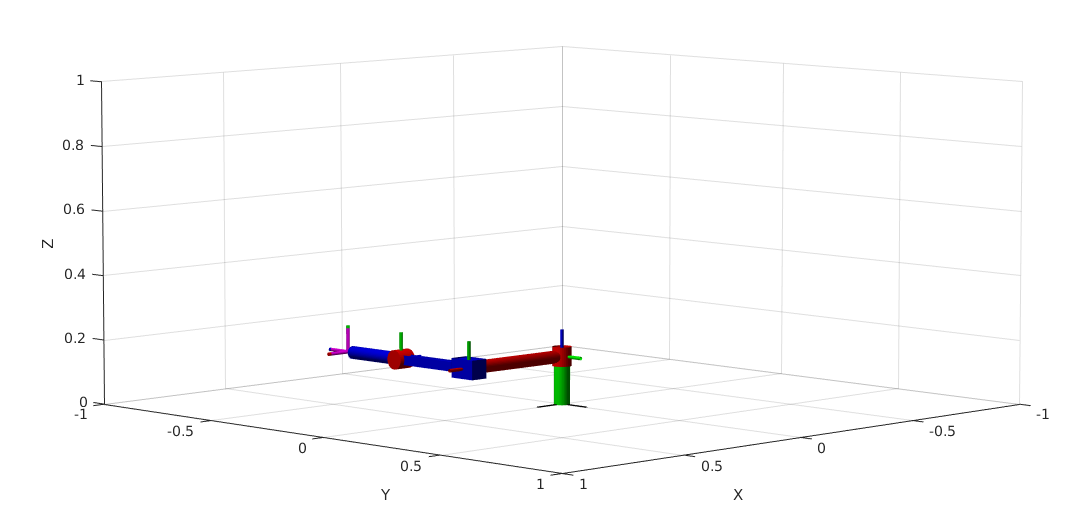
\includegraphics[keepaspectratio,width=0.5\textwidth]{1}
\caption{Visualization of the URDF of the PRP robot in the home configuration ($ q_1=0,q_2=0,\theta_3=0$)}
\end{figure}

\subsection{Denavit-Hartenberg parameters}

First of all, reference frames were assigned to each joint according to the DH convention:

\begin{figure}[h]
\centering
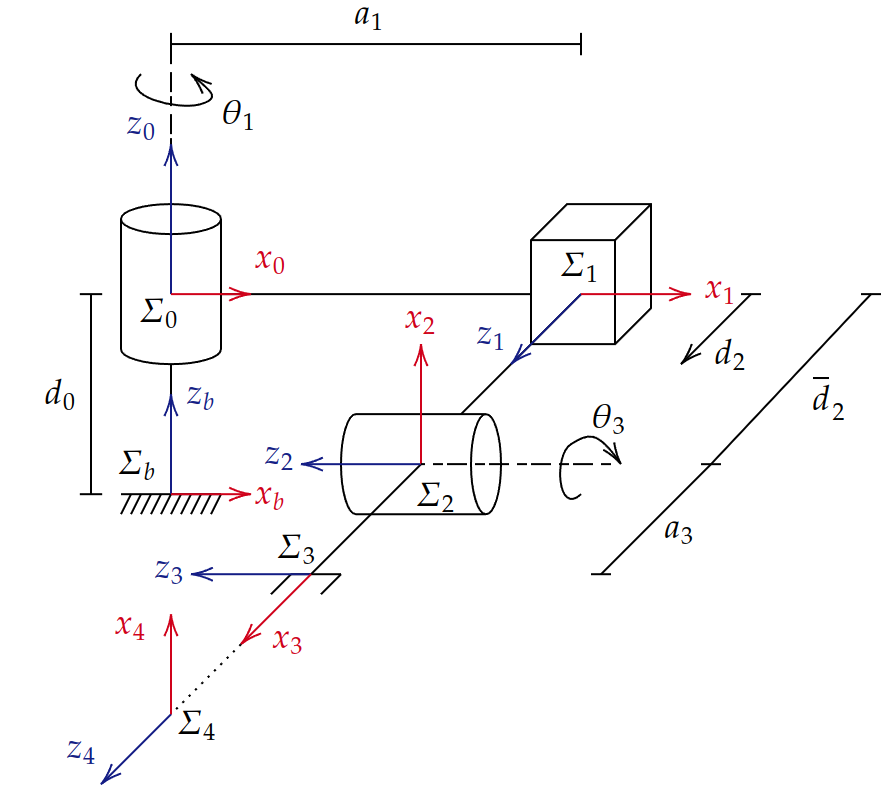
\includegraphics[keepaspectratio,width=0.45\textwidth]{2}
\caption{Reference frames assigned with the DH convention}
\end{figure}

Note that the DH frames do not correspond with the frames of the URDF model.

Then the DH parameter table was populated:

\begin{table}[h]
\centering
\begin{tabular}{c|c|c|c|c}
  & $a_i$ & $\alpha_i$       & $d_i$ & $\theta_i$      \\ \hline
0 & 0 & 0 & $d_0$ & 0\\
1 & $a_1$ & $\frac{\pi}{2}$  & 0     & $q_1 =  \theta_1$ \\
2 & 0     & $-\frac{\pi}{2}$ & $(q_2=d_2)+\overline d_2$ & $\frac{\pi}{2}$ \\
3 & $a_3$     & 0                & 0     & $(q_3=\theta_3)-\frac{\pi}{2}$\\
4 & 0 & $\frac{\pi}{2}$ & 0 & $\frac{\pi}{2}$
\end{tabular}
\end{table}

The first row is the fixed offset in the $z_b$ direction between world and frame $\Sigma_0$, while the last row is the fixed rotation that aligns the $z$ axis of the end-effector to the approach direction.

\newpage

Using the DH parameters, the transformation matrices between the frames were then computed. The transformation matrix between frame $i$ and frame $i-1$ is in the form:

\begin{align*}
T_{i-1}^i=\begin{bmatrix}
\cos(\theta_i)&-\sin(\theta_i)\cos(\alpha_i)&\sin(\theta_i)\sin(\alpha_i)&a_i\cos(\theta_i)\\
\sin(\theta_i)&\cos(\theta_i)\cos(\alpha_i)&-\cos(\theta_i)\sin(\alpha_i)&a_i\sin(\theta_i)\\
0&\sin(\alpha_i)&\cos(\alpha_i)&d_i\\
0&0&0&1
\end{bmatrix}
\end{align*}

The computed transformation matrices are then:
\begin{align*}
T_b^0&=\begin{bmatrix}
1 & 0 & 0 & 0\\ 0 & 1 & 0 & 0\\ 0 & 0 & 1 & d_0\\0 & 0 &0 &1
\end{bmatrix}
\;\;\;\;\;\;\;\;\;T_0^1=\begin{bmatrix}
C_1&0&S_1&a_1C_1\\
S_1&0&-C_1&a_1S_1\\
0&1&0&0\\
0&0&0&1
\end{bmatrix}\;\;\;\;\;\;\;\;\;
T_1^2=\begin{bmatrix}
0&0&-1&0\\
1&0&0&0\\
0&-1&0&q_2+\overline d_2\\
0&0&0&1
\end{bmatrix}\\T_2^3&=\begin{bmatrix}
C\left(q_3-\frac{\pi}{2}\right)&-S\left(q_3-\frac{\pi}{2}\right)&0&a_3C\left(q_3-\frac{\pi}{2}\right)\\
S\left(q_3-\frac{\pi}{2}\right)&C\left(q_3-\frac{\pi}{2}\right)&0&a_3S\left(q_3-\frac{\pi}{2}\right)\\
0&0&1&0\\
0&0&0&1
\end{bmatrix}=\begin{bmatrix}
S_3&C_3&0&a_3S_3\\-C_3&S_3&0&-a_3C_3\\0&0&1&0\\0&0&0&1
\end{bmatrix}\;\;\;\;\;\;\;\;\; T_3^4 = \begin{bmatrix}
0 & 0 & 1 & 0\\
1 & 0 & 0 & 0\\
0 & 1 & 0 & 0\\
0 & 0 & 0 & 1
\end{bmatrix}
\end{align*}

where $C_i$ and $S_i$ denote respectively $\cos(q_i)$ and $\sin(q_i)$.

\subsection{Direct kinematics}

The direct kinematics of the manipulator are obtained by chaining the above transformation matrices, thus obtaining a global transformation matrix from the end-effector to the base of the manipulator:

\begin{align*}
T_b^4&=T_b^0T_0^1T_1^2T_2^3T_3^4=\underset{T_b^1}{\underbrace{\begin{bmatrix}
C_1&0&S_1&a_1C_1\\
S_1&0&-C_1&a_1S_1\\
0&1&0&d_0\\
0&0&0&1
\end{bmatrix}}}T_1^2T_2^3T_3^4=\underset{T_b^2}{\underbrace{\begin{bmatrix}
0 & -S_1&-C_1&(q_2+\overline d_2)S_1+a_1C_1\\
0 & C_1&-S_1&-(q_2+\overline d_2)C_1+a_1S_1\\
1 & 0 & 0 & d_0\\
0&0&0&1
\end{bmatrix}}}T_2^3T_3^4\\
&=\underset{T_b^3}{\underbrace{\begin{bmatrix}
S_1C_3&-S_1S_3&-C_1&(q_2+\overline d_2)S_1+a_1C_1+a_3S_1C_3\\
-C_1C_3&C_1S_3&-S_1&-(q_2+\overline d_2)C_1+a_1S_1-a_3C_1C_3\\
S_3&C_3&0&d_0+a_3S_3\\
0&0&0&1
\end{bmatrix}}}T_3^4\\
&=\begin{bmatrix}
-S_1S_3 & -C_1 & S_1C_3 & (q_2+\overline d_2)S_1+a_1C_1+a_3S_1C_3\\
C_1S_3 & -S_1 & -C_1C_3 & -(q_2+\overline d_2)C_1+a_1S_1-a_3C_1C_3\\
C_3 & 0 & S_3 &d_0+a_3S_3\\
0&0&0&1 
\end{bmatrix} =\begin{bmatrix}
R_b^{4}&p_{4}\\
\overline 0 & 1
\end{bmatrix}
\end{align*}

\subsection{Inverse kinematics}

From the direct kinematics, the position of the end-effector is given by:

\begin{equation*}
p_{4}=\begin{pmatrix}
p_{4x}\\p_{4y}\\p_{4z}
\end{pmatrix}=\begin{pmatrix}
(q_2+\overline d_2)S_1+a_1C_1+a_3S_1C_3\\
-(q_2+\overline d_2)C_1+a_1S_1-a_3C_1C_3\\
d_0+a_3S_3
\end{pmatrix}
\end{equation*}

Therefore an expression for $q_3$ can immediately be derived:

\begin{equation*}
p_{4z}=d_0+a_3S_3\implies S_3=\frac{p_{4z}-d_0}{a_3}, C_3=\pm\sqrt{1-S_3^2}=\pm\sqrt{\frac{a_3^2-(p_{4z}-d_0)^2}{a_3^2}}\implies q_3^\pm=\atan2(S_3,\pm C_3)
\end{equation*}

$q_2$ is determined by applying summing and squaring to the position of the origin of frame $\Sigma_2$:

\begin{equation*}
p_2 = \begin{pmatrix}
p_{2x}\\p_{2y}\\p_{2z}
\end{pmatrix}=\begin{pmatrix}
(q_2+\overline d_2)S_1+a_1C_1\\
-(q_2+\overline d_2)C_1+a_1S_1\\
d_0
\end{pmatrix}
\end{equation*}
\begin{align*}
p_{2x}^2+p_{2y}^2&=S_1^2(q_2+\overline d_2)^2+a_1^2C_1^2+\cancel{2a_1(q_2+\overline d_2)S_1C_1}+C_1^2(q_2+\overline d_2)^2+a_1^2S_1^2-\cancel{2a_1(q_2+\overline d_2)S_1C_1}=\\
&=(q_2+\overline d_2)^2+a_1^2
\end{align*}

Therefore $q_2$ is given by the solution of the quadratic equation:

\begin{equation*}
q_2^2+2\overline d_2q_2+a_2-p_{2x}^2-p_{2y}^2=0
\end{equation*}

which is:

\begin{equation*}
q_{2,12}=-\frac{\cancel{2}\overline d_2\pm\sqrt{\cancel{4\overline d_2^2}-\cancel{4}(a_1^2+\cancel{\overline d_2}-p_{2x}^2-p_{2y}^2)}}{\cancel{2}}=-\overline d_2\pm\sqrt{p_{2x}^2+p_{2y}^2-a_1^2}
\end{equation*}

To choose the solution, both are computed and the correct one will be the one that satisfies joint limits.

To choose the correct sign for $q_3$, $q_2$ is recomputed by summing and squaring the $x$ and $y$ components of $p_3$:

\begin{align*}
p_{3x}^2+p_{3y}^2&=S_1^2(q_2+\overline d_2)^2+a_1^2C_1^2+a_3^2S_1^2C_3^2+\cancel{2a_1(q_2+\overline d_2)S_1C_1}+2a_3(q_2+\overline d_2)S_1^2C_3+\cancel{2a_1a_3S_1C_1C_3}\\&+C_1^2(q_2+\overline d_2)^2+a_1^2S_1^2+a_3^2C_1^2C_3^2-\cancel{2a_1(q_2+\overline d_2)S_1C_1}+2a_3(q_2+\overline d_2)C_1^2C_3-\cancel{2a_1a_3S_1C_1C_3}=\\
&=(q_2+\overline d_2)^2+a_1^2+a_3^2C_3^2+2a_3(q_2+\overline d_2)C_3
\end{align*}

and therefore:

\begin{equation*}
q_{2,12}= -a_3C_3-\overline d_2\pm\sqrt{p_{4x}^2+p_{4y}^2-a_1^2}
\end{equation*}

By computing the four possible solutions and checking which one is equal to the one obtained previously, it is possible to determine the correct sign for $C_3$ and therefore the correct value for $q_3$.

Finally, $q_1$ is determined by solving the system of equations:

\begin{equation*}
\begin{cases}
p_{2x}=(q_2+\overline d_2)S_1+a_1C_1\\
p_{2y}=-(q_2+\overline d_2)C_1+a_1S_1
\end{cases}
\end{equation*}

in the unknowns $C_1$ and $S_1$. The system yields:

\begin{equation*}
C_1 = \frac{a_1p_{2x}-(q_2+\overline d_2)p_{2y}}{(q_2+\overline d_2)^2+a_1^2}, S_1=\frac{p_{2x}-a_1C_1}{(q_2+\overline d_2)}\implies q_1=\atan2(S_1,C_1)
\end{equation*}

For the orientation $o_4$ of the end-effector, the angles $\alpha,\beta$ and $\gamma$ can be derived by equating the rotation matrix $R_b^4$ to the rotation matrix that expresses a $ZXZ$ Euler angle rotation:

\begin{equation*}
\begin{bmatrix}
-S_1S_3 & -C_1 & S_1C_3\\
C_1S_3 & -S_1 & -C_1C_3\\
C_3 & 0 & S_3
\end{bmatrix}=\begin{bmatrix}
C_\alpha C_\gamma-C_\beta S_\alpha S_\gamma & -C_\alpha S_\gamma-C_\beta C_\gamma S_\alpha & S_\alpha S_\beta\\
S_\alpha C_\gamma+C_\beta C_\alpha S_\gamma & -S_\alpha S_\gamma-C_\beta C_\gamma C_\alpha & -C_\alpha S_\beta\\
S_\beta S_\gamma & C_\gamma S_\beta & C_\beta
\end{bmatrix}
\end{equation*}

\begin{equation*}
\begin{cases}
S_\alpha S_\beta = S_1C_3, -C_\alpha S_\beta = -C_1C_3 \implies S_\alpha=S_1,C_\alpha=C_1&\implies \alpha = q_1\\ 
C_\beta = S_3&\implies \beta = \frac{\pi}{2}-q_3\\
S_\beta S_\gamma = C_3\implies S_\gamma = 1&\implies \gamma = \frac{\pi}{2}
\end{cases}
\implies o_{4} = \begin{pmatrix}
\alpha\\\beta\\\gamma
\end{pmatrix}=\begin{pmatrix}
q_1\\\frac{\pi}{2}-q_3\\ \frac{\pi}{2}
\end{pmatrix}
\end{equation*}

\subsection{Analytical Jacobian}

The lines of the analytical Jacobian are the gradients of the pose (position and orientation) of the end-effector with respect to the joint variables:

\begin{align*}
\nabla p_x&=\begin{bmatrix}
\frac{\partial p_x}{\partial q_1}&\frac{\partial p_x}{\partial q_2}&\frac{\partial p_x}{\partial q_3}
\end{bmatrix}=\begin{bmatrix}
(q_2+\overline d_2)C_1-a_1S_1+a_3C_3C_1 &  S_1 & -a_3S_1S_3
\end{bmatrix}\\
\nabla p_y&=\begin{bmatrix}
\frac{\partial p_y}{\partial q_1}&\frac{\partial p_y}{\partial q_2}&\frac{\partial p_y}{\partial q_3}
\end{bmatrix}=\begin{bmatrix}
(q_2+\overline d_2)S_1+a_1C_1+a_3S_1C_3 &  -C_1 & a_3S_1S_3
\end{bmatrix}\\
\nabla p_z&=\begin{bmatrix}
\frac{\partial p_z}{\partial q_1}&\frac{\partial p_z}{\partial q_2}&\frac{\partial p_z}{\partial q_3}
\end{bmatrix}=\begin{bmatrix}
0 & 0 & a_3C_3
\end{bmatrix}\\
\nabla \alpha&=\begin{bmatrix}
\frac{\partial\alpha}{\partial q_1}&\frac{\partial\alpha}{\partial q_2}&\frac{\partial\alpha}{\partial q_3}
\end{bmatrix}=\begin{bmatrix}
1 & 0 & 0
\end{bmatrix}\\
\nabla \beta&=\begin{bmatrix}
\frac{\partial\beta}{\partial q_1}&\frac{\partial\alpha}{\partial q_2}&\frac{\partial\beta}{\partial q_3}
\end{bmatrix}=\begin{bmatrix}
0 & 0 & -1
\end{bmatrix}\\
\nabla \gamma&=\begin{bmatrix}
\frac{\partial\gamma}{\partial q_1}&\frac{\partial\gamma}{\partial q_2}&\frac{\partial\gamma}{\partial q_3}
\end{bmatrix}=\begin{bmatrix}
0 & 0 & 0
\end{bmatrix}
\end{align*}

\newpage

Therefore the analytical Jacobian is:

\begin{equation*}
J_A = \begin{bmatrix}
\nabla p_x\\\nabla p_y\\\nabla p_z\\\nabla\alpha\\\nabla\beta\\\nabla\gamma
\end{bmatrix}=\begin{bmatrix}
(q_2+\overline d_2)C_1-a_1S_1+a_3C_3C_1 &  S_1 & -a_3S_1S_3\\
(q_2+\overline d_2)S_1+a_1C_1+a_3S_1C_3 &  -C_1 & a_3C_1S_3\\
0 & 0 & a_3C_3\\
1 & 0 & 0\\
0 & 0 & -1\\
0 & 0 & 0
\end{bmatrix}\implies\begin{bmatrix}
\dot p_4\\\dot o_4\end{bmatrix} = J_A\dot q
\end{equation*}

where $\dot q = \begin{bmatrix}
\dot q_1 & \dot q_2 & \dot q_3
\end{bmatrix}^T$.

\subsection{Geometric Jacobian}

The $i$-th column of the geometric Jacobian ($i=0,\dots,n-1$) is constructed as follows:

\begin{equation*}
J_{Gi} = \begin{bmatrix}
z_i\cross (p_4-p_i)\\ z_i
\end{bmatrix}\;\;\;\text{(revolute joint)}\;\;\;\;\;\;\;\;\;\;\;\;
J_{Gi} = \begin{bmatrix}
z_i\\ 0\\0\\0
\end{bmatrix}\;\;\;\text{(prismatic joint)}
\end{equation*}

where $p_4$ is the position of the end-effector, $p_i$ is the position of frame $i$ and $z_i$ is the direction of the $z$ axis of frame $i$, all with respect to the base frame.

So:

\begin{align*}
p_2 &=\begin{bmatrix}
S_1(q_2+\overline d_2)+a_1C_1\\
-C_1(q_2+\overline d_2)+a_1S_1\\
d_0
\end{bmatrix},z_2=\begin{bmatrix}
-C_1\\-S_1\\0
\end{bmatrix}\implies J_{G2}=\begin{bmatrix}
-a_3S_1S_3 & a_3C_1C_3 & a_3C_3 & -C_1 & -S_1 & 0
\end{bmatrix}^T\\
p_1 &= \begin{bmatrix}
a_1C_1\\a_1S_1\\d_0
\end{bmatrix},z_1=\begin{bmatrix}
S_1\\-C_1\\0
\end{bmatrix}\implies J_{G1}=\begin{bmatrix}
S_1&-C_1&0&0&0&0
\end{bmatrix}^T\\
p_0&=\begin{bmatrix}
0\\0\\d_0
\end{bmatrix},z_0=\begin{bmatrix}
0\\0\\1
\end{bmatrix}\implies J_{G0} = \begin{bmatrix}
C_1(q_2+\overline d_2)-a_1S_1+a_3C_1C_3 & S_1(q_2+\overline d_2)+a_1C_1+a_3S_1C_3 & 0 & 0 & 0 & 1
\end{bmatrix}^T
\end{align*}

Finally:

\begin{equation*}
J_G = \begin{bmatrix}
C_1(q_2+\overline d_2)-a_1S_1+a_3C_1C_3 & S_1&-a_3S_1S_3  \\
S_1(q_2+\overline d_2)+a_1C_1+a_3S_1C_3 &-C_1& a_3C_1C_3  \\
  0&0& a_3C_3 \\
0&0 & -C_1\\
0&0&-S_1 \\
    1& 0&0
\end{bmatrix}\implies \begin{bmatrix}
\dot p_3\\ \omega_3
\end{bmatrix}=J_G\dot q
\end{equation*}

As expected, the rows of the geometric Jacobian related to linear velocity are the same ones found in the analytical Jacobian.

\subsection{Relationship between JG and JA}

The geometric and analytical Jacobians are related by the following relationship:

\begin{equation*}
J_G = T_A(\Phi)J_A=\begin{bmatrix}
I&0\\0&T(\Phi)
\end{bmatrix}J_A
\end{equation*}

Therefore:

\begin{equation*}
\begin{bmatrix}
0&0 & -C_1\\
0&0&-S_1 \\
    1& 0&0
\end{bmatrix} = T(\Phi)\begin{bmatrix}
1 & 0 & 0\\
0 & 0 & -1\\
0 & 0 & 0
\end{bmatrix}\implies T(\Phi) = \begin{bmatrix}
0&0 & -C_1\\
0&0&-S_1 \\
    1& 0&0
\end{bmatrix}\begin{bmatrix}
1 & 0 & 0\\
0 & 0 & -1\\
0 & 0 & 0
\end{bmatrix}^{\dagger} = \begin{bmatrix}
0 & C_1 & 0\\ 0 & S_1 & 0\\ 1 & 0 & 0
\end{bmatrix}
\end{equation*}

where $^\dagger$ denotes the Moore-Penrose pseudoinverse.

\newpage

\section{Assignment 2}

To compute both the kinetic and potential energy, the positions of the centres of mass of each link are needed. With respect to each frame $\Sigma_i$ attached to link $i$:

\begin{equation*}
p_{l_1}^1=\begin{bmatrix}
-\frac{h_1}{2}\\0\\0
\end{bmatrix}\;\;\;\;\;\;\;\;\;p_{l_2}^2=\begin{bmatrix}
0\\\frac{a_2}{2}\\0
\end{bmatrix}\;\;\;\;\;\;\;\;\;p_{l_3}^3=\begin{bmatrix}
-\frac{h_3}{2}\\0\\0
\end{bmatrix}
\end{equation*}

Using the transformation matrices obtained with direct kinematics, the positions of the centres of mass with respect to the base frame $\Sigma_b$ are:

\begin{equation*}
p_{l_1}=R_b^1p_{l_1}^1+p_1=\begin{bmatrix}
\left(a_1-\frac{h_1}{2}\right)C_1\\\left(a_1-\frac{h_1}{2}\right)S_1\\d_0
\end{bmatrix}\;\;\;\;\;\;\;\;\;p_{l_2}=R_b^2p_{l_2}^2+p_2=\begin{bmatrix}
\left(q_2+\overline d_2-\frac{a_2}{2}\right)S_1+a_1C_1\\-\left(q_2+\overline d_2-\frac{a_2}{2}\right)C_1+a_1S_1\\d_0
\end{bmatrix}
\end{equation*}
\begin{equation*}
p_{l_3}=R_b^3p_{l_3}^3+p_3=\begin{bmatrix}
(q_2+\overline d_2)S_1+a_1C_1+\left(a_3-\frac{h_3}{2}\right)S_1C_3\\ -(q_2+\overline d_2)C_1+a_1S_1-\left(a_3-\frac{h_3}{2}\right)C_1C_3\\d_0+\left(a_3-\frac{h_3}{2}\right)S_3
\end{bmatrix}
\end{equation*}


\subsection{Compute the kinetic energy}

The total kinetic energy for an open-chain manipulator is:

\begin{equation*}
\T(q,\dot q)=\frac{1}{2}\dot q^TB(q)\dot q\;\;\;\;\;\;\;B(q)=\sum\limits_{i=1}^n(m_{l_i}(J_P^{l_i})^TJ_P^{l_i}+(J_O^{l_i})^TR_b^iI_{l_i}^i{R_b^i}^TJ_O^{l_i})
\end{equation*}

where $B(q)$ is the inertia matrix, $I_{l_i}^i$ are the inertia tensors with respect to $\Sigma_i$, $J_P^{l_i}$ and $J_O^{l_i}$ are the linear and angular partial Jacobian matrices and $R_b^i$ are the rotation matrices that bring frame $\Sigma_i$ to frame $\Sigma_b$.

The inertia tensors are obtained with Steiner's theorem:

\begin{align*}
I_{l_1}^1 &= I_{l_1}^{C_1}+m_{l_1}S^T(p_{l_1}^1)S(p_{l_1}^1)\\
&=m_{l_1}\begin{bmatrix}
\frac{1}{2}(r_1^2)&0&0\\
0&\frac{1}{2}(3r_1^2+h_1^2)&0\\
0&0&\frac{1}{2}(3r_1^2+h_1^2)
\end{bmatrix}+m_{l_1}\begin{bmatrix}
0&0&0\\0&\frac{h_1^2}{4}&0\\0&0&\frac{h_1^2}{4}
\end{bmatrix}\\&=\frac{1}{2}m_{l_1}\begin{bmatrix}
r_1^2&0&0\\
0&3r_1^2+\frac{3h_1^2}{2}&0\\
0&0&3r_1^2+\frac{3h_1^2}{2}
\end{bmatrix}\\
I_{l_2}^2 &= I_{l_2}^{C_2}+m_{l_2}S^T(p_{l_2}^2)S(p_{l_2}^2)\\
&=m_{l_2}\begin{bmatrix}
\frac{1}{12}(b_2^2+c_2^2)&0&0\\
0&\frac{1}{12}(a_2^2+c_2^2)&0\\
0&0&\frac{1}{12}(a_2^2+b_2^2)
\end{bmatrix}+m_{l_2}\begin{bmatrix}
\frac{a_2^2}{4}&0&0\\0&0&0\\0&0&\frac{a_2^2}{4}
\end{bmatrix}\\
&=\frac{1}{12}m_{l_2}\begin{bmatrix}
3a_2^2+b_2^2+c_2^2&0&0\\0&a_2^2+c_2^2&0\\0&0&4a_2^2+b_2^2
\end{bmatrix}\\
I_{l_3}^3 &= I_{l_3}^{C_3}+m_{l_3}S^T(p_{l_3}^3)S(p_{l_3}^3)\\
&=m_{l_3}\begin{bmatrix}
\frac{1}{2}(r_3^2)&0&0\\
0&\frac{1}{2}(3r_3^2+h_3^2)&0\\
0&0&\frac{1}{2}(3r_3^2+h_3^2)
\end{bmatrix}+m_{l_3}\begin{bmatrix}
0&0&0\\0&\frac{h_3^2}{4}&0\\0&0&\frac{h_3^2}{4}
\end{bmatrix}\\
&=\frac{1}{2}m_{l_3}\begin{bmatrix}
r_3^2&0&0\\
0&3r_3^2+\frac{3}{2}h_3^2&0\\
0&0&3r_3^2+\frac{3}{2}h_3^2
\end{bmatrix}
\end{align*}

The links are assumed to be made up of an homogeneous material, specifically aluminium. Therefore the mass $m_{l_i}$ of link $i$ is $m_{l_i}=\rho V_{l_i}$, where $\rho=2710\;kg/m^3$ is the density of aluminium and $V_{l_i}$ is the volume of link $i$.

\newpage

The partial Jacobian matrices are constructed as follows:

\begin{align*}
J_P^{l_i}&=\begin{bmatrix}
j_{P1}^{l_i}&\dots&j_{Pj}^{l_i}& 0&\dots&0
\end{bmatrix}\;\;\text{where }j_{Pj}^{l_i}=\begin{cases}
z_{j-1}&\text{prismatic joint}\\
z_{j-1}\cross(p_{l_i}-p_{j-1})&\text{revolute joint}\\
\end{cases}\\
J_O^{l_i}&=\begin{bmatrix}
j_{O1}^{l_i}&\dots&j_{Oj}^{l_i}& 0&\dots&0
\end{bmatrix}\;\;\text{where }j_{Oj}^{l_i}=\begin{cases}
0&\text{prismatic joint}\\
z_{j-1}&\text{revolute joint}\\
\end{cases}
\end{align*}

where $p_{j-1}$ is the position vector of the origin of frame $\Sigma_{j-1}$ and $z_{j-1}$ is the unit vector of axis $z$ of frame $\Sigma_{j-1}$, all with respect of $\Sigma_b$.

\hspace{-0.75cm}
\begin{minipage}[h]{0.6\textwidth}
\begin{align*}
J_P^{l_1}&=\begin{bmatrix}
j_{P1}^{l_1} & 0 & 0
\end{bmatrix}=\begin{bmatrix}
-S_1\left(a_1 -\frac{h_1}{2}\right)&0&0\\C_1\left(a_1 -\frac{h_1}{2}\right)&0&0\\0&0&0
\end{bmatrix}\\
j_{P1}^{l_1}&=z_0\cross(p_{l_1}-p_{0})=\begin{bmatrix}
-S_1\left(a_1 -\frac{h_1}{2}\right)&C_1\left(a_1 -\frac{h_1}{2}\right)&0\end{bmatrix}^T\\\\
J_P^{l_2}&=\begin{bmatrix}
j_{P1}^{l_2} & j_{P2}^{l_2} & 0
\end{bmatrix}=\begin{bmatrix}
\left(d_2 + q_2-\frac{a_2}{2}\right)C_1&  S_1& 0\\
\left(d_2 + q_2-\frac{a_2}{2}\right)S_1& -C_1& 0\\
                                    0&    0& 0
\end{bmatrix}\\
j_{P1}^{l_2}&=z_0\cross(p_{l_2}-p_{0})=\begin{bmatrix}
\left(d_2 + q_2-\frac{a_2}{2}\right)C_1 &
\left(d_2 + q_2-\frac{a_2}{2}\right)S_1 &
                                    0
\end{bmatrix}^T\\
j_{P2}^{l_2}&=z_1=\begin{bmatrix}
 S_1&-C_1&   0
\end{bmatrix}^T\\\\
J_P^{l_3}&=\begin{bmatrix}
j_{P1}^{l_3} & j_{P2}^{l_3} &j_{P3}^{l_3}
\end{bmatrix}=\begin{bmatrix}
C_1C_3\left(a_3-\frac{h_3}{2}\right)&S_1&  S_1S_3\left(a_3-\frac{h_3}{2}\right)\\
S_1C_3\left(a_3-\frac{h_3}{2}\right)&-C_1& -C_1S_3\left(a_3-\frac{h_3}{2}\right)\\ 
                                      0  &  0  &             C_3\left(a_3-\frac{h_3}{2}\right)         
\end{bmatrix}\\
j_{P1}^{l_3}&=z_0\cross(p_{l_3}-p_{0})=\begin{bmatrix}
C_1C_3\left(a_3-\frac{h_3}{2}\right)&
S_1C_3\left(a_3-\frac{h_3}{2}\right)&
                                      0
\end{bmatrix}^T\\
j_{P2}^{l_3}&=z_1=\begin{bmatrix}
 S_1&
 -C_1&
    0
\end{bmatrix}^T\\
j_{P3}^{l_3}&=z_2\cross(p_{l_3}-p_{2})=\begin{bmatrix}
   S_1S_3\left(a_3-\frac{h_3}{2}\right)&
-C_1S_3\left(a_3-\frac{h_3}{2}\right)&
             C_3\left(a_3-\frac{h_3}{2}\right) 
\end{bmatrix}^T
\end{align*}
\end{minipage}
\hspace{0.25cm}
\begin{minipage}[h]{0.3\textwidth}
\begin{align*}
J_O^{l_1}&=\begin{bmatrix}
j_{O1}^{l_1} & 0 & 0
\end{bmatrix}=\begin{bmatrix}
0&0&0\\0&0&0\\1&0&0
\end{bmatrix}\\
j_{O1}^{l_1}&=z_0=\begin{bmatrix}
0&0&1
\end{bmatrix}^T\\\\
J_O^{l_2}&=\begin{bmatrix}
j_{O1}^{l_2} & j_{O2}^{l_2} & 0
\end{bmatrix}=\begin{bmatrix}
0&0&0\\0&0&0\\1&0&0
\end{bmatrix}\\
j_{O1}^{l_2}&=z_0=\begin{bmatrix}
0&0&1
\end{bmatrix}^T\\
j_{O2}^{l_2}&=\begin{bmatrix}
0&0&0
\end{bmatrix}^T\\\\
J_O^{l_3}&=\begin{bmatrix}
j_{O1}^{l_3} & j_{O2}^{l_3} & j_{O3}^{l_3}
\end{bmatrix}=\begin{bmatrix}
0&0&-C_1\\0&0&-S_1\\1&0&0
\end{bmatrix}\\
j_{O1}^{l_3}&=z_0=\begin{bmatrix}
0&0&1
\end{bmatrix}^T\\
j_{O2}^{l_3}&=\begin{bmatrix}
0&0&0
\end{bmatrix}^T\\
j_{O3}^{l_3}&=z_2=\begin{bmatrix}
-C_1&-S_1&0
\end{bmatrix}^T
\end{align*}
\end{minipage}

So the inertial matrices of each joint are:

\begin{align*}
B_1(q)&=m_{l_1}(J_P^{l_1})^TJ_P^{l_1}+(J_O^{l_1})^TR_b^1I_{l_1}^1{R_b^1}^TJ_O^{l_1}\\
&=m_{l_1}\begin{bmatrix}
\frac{1}{2}((a_1-h_1)^2+r_1^2)& 0& 0\\ *& 0& 0\\ *& *& 0
 \end{bmatrix}\\
B_2(q)&=m_{l_2}(J_P^{l_2})^TJ_P^{l_2}+(J_O^{l_2})^TR_b^2I_{l_2}^2{R_b^2}^TJ_O^{l_2}\\
&=m_{l_2}\begin{bmatrix}
a_1^2+\left(d_2+q_2-\frac{1}{2}a_2\right)^2+\frac{1}{12}\left(a_2^2+c_2^2\right)&-a_1&0\\
*& 1 & 0\\
*&*&0
\end{bmatrix}\\
B_3(q)&=m_{l_3}(J_P^{l_3})^TJ_P^{l_3}+(J_O^{l_3})^TR_b^3I_{l_3}^3{R_b^3}^TJ_O^{l_3}\\
&=m_{l_3}\begin{bmatrix}
a_1^2 + \left(d_2+q_2-\left(\frac{1}{2}h_3-a_3\right)C_3\right)^2+\frac{1}{12}(h_3^2+r_3^2) & -a_1 & \frac{1}{2}a_1(2a_3-h_3)S_3\\
* & 1 & -\frac{1}{2}(2a_3-h_3)S_3\\
* & * & a_3^2-a_3h_3+h_3^2+\frac{1}{2}r_3^2
\end{bmatrix}
\end{align*} 
     
\newpage

So the overall inertia matrix is:

\begin{align*}
B(q) &= B_1(q)+B_2(q)+B_3(q)\\&= \begin{bmatrix}
K& -a_1( m_{l_2} + m_{l_3}) & \frac{1}{2}m_{l_3}a_1(2a_3-h_3)S_3\\
* & m_{l_2} + m_{l_3} & -\frac{1}{2}m_{l_3}(2a_3-h_3)S_3\\
* & * & a_3^2-a_3h_3+h_3^2+\frac{1}{2}r_3^2
\end{bmatrix}\\&=\begin{bmatrix}
0.4904q_2 + 0.05885C_3 + 0.0474C_3^2 + 0.1962q_2C_3 + 0.8173q_2^2 + 0.4796&          -0.6196&  0.03923S_3\\
 * &          1.549 & -0.09808S_3\\ *& * &0.04757
\end{bmatrix}
\end{align*}

with :

\begin{align*}
K&=\frac{1}{2}m_{l_1}\left((a_1-h_1)^2+r_1^2\right)+m_{l_2}\left(a_1^2+\left(d_2+q_2-\frac{1}{2}a_2\right)^2+\frac{1}{12}\left(a_2^2+c_2^2\right)\right)\\&+m_{l_3}\left(a_1^2 + \left(d_2+q_2-\left(\frac{1}{2}h_3-a_3\right)C_3\right)^2+\frac{1}{12}(h_3^2+r_3^2)\right)
\end{align*}

Finally, the kinetic energy is given by:

\begin{align*}
\T(q,\dot q) = \frac{1}{2}\dot q^TB(q)\dot q
&=0.0237\dot q_1^2C_3^2 - 0.6196\dot q_1\dot q_2 + 0.3549\dot q_1^2 q_2 + 0.248\dot q_1^2 + 0.7745\dot q_2^2 + 0.02378\dot q_3^2 \\&+ 0.7745\dot q_1^2q_2^2 + 0.02942\dot q_1^2C_3 + 0.03923\dot q_1 \dot q_3S_3 - 0.09808\dot q_2\dot q_3S_3 + 0.09808\dot q_1^2q_2C_3
\end{align*}

The symbolic expression is not reported for space reasons.

\subsection{Compute the potential energy}

The potential energy is given by:

\begin{equation*}
\U(q)=-\sum\limits_{i=1}^nm_{l_i}g_0^Tp_{l_i}
\end{equation*}

where $g_0=\begin{bmatrix}
0&0&-g
\end{bmatrix}^T$ is the gravity acceleration vector in the base frame $\Sigma_b$.

So:

\begin{align*}
\U_1&=-m_{l_1}gd_0\\
\U_2&=-m_{l_2}gd_0\\
\U_3(q)&=-m_{l_3}g\left(d_0+\left(a_3-\frac{h_3}{2}\right)S_3\right)
\end{align*}

Finally:

\begin{equation*}
\U(q) = -(\U_1+\U_2+\U_3(q))=\left[(m_{l_1}+m_{l_2}+m_{l_3})d_0+m_{l_3}\left(a_3-\frac{h_3}{2}\right)S_3\right]g = 0.9621S_3 + 4.033
\end{equation*}

\newpage

\section{Assignment 3}

\subsection{Equations of motion}

The equations of motion for an open chain robotic manipulator are:

\begin{equation*}
B(q)\ddot q+C(q,\dot q)\dot q+F_v\dot q+F_ssign(\dot q)+g(q)=\tau-J^T(q)h_e
\end{equation*}

Ignoring the contributions related to frictions and the external wrench ($F_v,F_s,he$), the equations reduce to:

\begin{equation*}
B(q)\ddot q+C(q,\dot q)\dot q+g(q)=\tau
\end{equation*}

where $\tau$ is the command torque, $C(q,\dot q)$ is the Coriolis matrix and $g(q)$ is the gravity term, which is given by:

\begin{equation*}
g_i(q)=-\sum\limits_{j=1}^nm_{l_i}g_0^Tj_{Pi}^{l_j}(q)\rightarrow g(q)=\begin{bmatrix}
0\\0\\m_{l_3}g\left(a_3-\frac{1}{2}h_3\right)C_3
\end{bmatrix}=\begin{bmatrix}
0\\0\\ -0.9621C_3
\end{bmatrix}
\end{equation*}

The $c_{ij}$ elements of $C(q,\dot q)$ are:

\begin{equation*}
c_{ij}=\sum\limits_{k=1}^n\frac{1}{2}\left(\frac{\partial b_{ij}}{\partial q_k}+\frac{\partial b_{ik}}{\partial q_j}-\frac{\partial b_{jk}}{\partial q_i}\right)\dot q_k
\end{equation*}

where $b_{ij},b_{ik}$ and $b_{jk}$ are the elements of the inertial matrix $B(q)$. The derivatives of the $B(q)$ matrix are:

\begin{align*}
\frac{\partial B}{\partial q_1}&=\begin{bmatrix}
0&0&0\\ *&0&0\\ *&*&0
\end{bmatrix}\\
\frac{\partial B}{\partial q_2}&=\begin{bmatrix}
3.098q_2+0.1962C_3+0.7099&0&0\\ *&0&0\\ *&*&0
\end{bmatrix}\\
\frac{\partial B}{\partial q_3}&=\begin{bmatrix} 
- 0.0948S_3C_3 - 0.05885S_3 - 0.1962q_2S_3&                0& 0.03923C_3\\
                                                     *&                0& -0.09808C_3\\
                                         *& *&                0
\end{bmatrix}
\end{align*}

So the $c_{ij}$ components are:

\begin{align*}
c_{11}&=\frac{1}{2}\left(\frac{\partial b_{11}}{\partial q_1}+\frac{\partial b_{11}}{\partial q_1}-\frac{\partial b_{11}}{\partial q_1}\right)\dot q_1+\frac{1}{2}\left(\frac{\partial b_{11}}{\partial q_2}+\frac{\partial b_{12}}{\partial q_1}-\frac{\partial b_{12}}{\partial q_1}\right)\dot q_2+\frac{1}{2}\left(\frac{\partial b_{11}}{\partial q_3}+\frac{\partial b_{13}}{\partial q_1}-\frac{\partial b_{13}}{\partial q_1}\right)\dot q_3\\
&=\frac{1}{2}m_{l_2}(2d_2+2q_2-a_2)\dot q_2+m_{l_3}S_3C_3(a_3h_3-a_3^2-h_3^2-r_3^2)\dot q_3\\
c_{12}&=
\frac{1}{2}\left(\frac{\partial b_{12}}{\partial q_1}+\frac{\partial b_{11}}{\partial q_2}-\frac{\partial b_{21}}{\partial q_1}\right)\dot q_1+
\frac{1}{2}\left(\frac{\partial b_{12}}{\partial q_2}+\frac{\partial b_{12}}{\partial q_2}-\frac{\partial b_{22}}{\partial q_1}\right)\dot q_2+
\frac{1}{2}\left(\frac{\partial b_{12}}{\partial q_3}+\frac{\partial b_{13}}{\partial q_2}-\frac{\partial b_{23}}{\partial q_1}\right)\dot q_3\\
&=0.5\dot q_1\dot q_2(3.098q_2 + 0.1962C_3 + 0.7099)\\
c_{13}&=
\frac{1}{2}\left(\frac{\partial b_{13}}{\partial q_1}+\frac{\partial b_{11}}{\partial q_3}-\frac{\partial b_{31}}{\partial q_1}\right)\dot q_1+
\frac{1}{2}\left(\frac{\partial b_{13}}{\partial q_2}+\frac{\partial b_{12}}{\partial q_3}-\frac{\partial b_{32}}{\partial q_1}\right)\dot q_2+
\frac{1}{2}\left(\frac{\partial b_{13}}{\partial q_3}+\frac{\partial b_{13}}{\partial q_3}-\frac{\partial b_{33}}{\partial q_1}\right)\dot q_3\\
&=0.03923C_3\dot q_3^2 - 0.5\dot q_1(0.0948S_3C_3 + 0.05885S_3 + 0.1962q_2S_3)\dot q_3\\
c_{22}&=
\frac{1}{2}\left(\frac{\partial b_{22}}{\partial q_1}+\frac{\partial b_{21}}{\partial q_2}-\frac{\partial b_{21}}{\partial q_2}\right)\dot q_1+
\frac{1}{2}\left(\frac{\partial b_{22}}{\partial q_2}+\frac{\partial b_{22}}{\partial q_2}-\frac{\partial b_{22}}{\partial q_2}\right)\dot q_2+
\frac{1}{2}\left(\frac{\partial b_{22}}{\partial q_3}+\frac{\partial b_{23}}{\partial q_2}-\frac{\partial b_{23}}{\partial q_2}\right)\dot q_3\\
&=0\\
c_{23}&=
\frac{1}{2}\left(\frac{\partial b_{23}}{\partial q_1}+\frac{\partial b_{21}}{\partial q_3}-\frac{\partial b_{31}}{\partial q_2}\right)\dot q_1+
\frac{1}{2}\left(\frac{\partial b_{23}}{\partial q_2}+\frac{\partial b_{22}}{\partial q_3}-\frac{\partial b_{32}}{\partial q_2}\right)\dot q_2+
\frac{1}{2}\left(\frac{\partial b_{23}}{\partial q_3}+\frac{\partial b_{23}}{\partial q_3}-\frac{\partial b_{33}}{\partial q_2}\right)\dot q_3\\
&=0\\
c_{33}&=
\frac{1}{2}\left(\frac{\partial b_{33}}{\partial q_1}+\frac{\partial b_{31}}{\partial q_3}-\frac{\partial b_{31}}{\partial q_3}\right)\dot q_1+
\frac{1}{2}\left(\frac{\partial b_{33}}{\partial q_2}+\frac{\partial b_{32}}{\partial q_3}-\frac{\partial b_{32}}{\partial q_3}\right)\dot q_2+
\frac{1}{2}\left(\frac{\partial b_{33}}{\partial q_3}+\frac{\partial b_{33}}{\partial q_3}-\frac{\partial b_{33}}{\partial q_3}\right)\dot q_3\\
&=0\\
\end{align*}

\newpage

So the equations of motion are:

\begin{equation*}
B(q)\ddot q+C(q,\dot q)\dot q+g(q)=\tau
\end{equation*}

\begin{equation*}
\resizebox{\textwidth}{!}{$
\begin{bmatrix}
\tau_1\\\tau_2\\\tau_3
\end{bmatrix}=
\begin{bmatrix}
0.496\ddot q_1 - 0.6196\ddot q_2 + 0.7099\ddot q_1q_2 + 0.7099\dot q_1\dot q_2^2 + 1.549\ddot q_1q_2^2 + 0.05885\ddot q_1C_3 + 0.03923d\dot q_3S_3 + 0.0474\ddot q_1C_3^2 + 0.03923\dot q_3^3C_3 + 0.1962\ddot q_1q_2C_3 - 0.0474\dot q_1\dot q_3^2sin(2.0q_3) + 0.1962\dot q_1\dot q_2^2C_3 - 0.05885\dot q_1\dot q_3^2S_3 + 3.098\dot q_1\dot q_2^2q_2 - 0.1962\dot q_1\dot q_3^2q_2S_3\\ 0.5\dot q_2(3.098q_2 + 0.1962C_3 + 0.7099)\dot q_1^2 - 0.6196\ddot q_1 + 1.549\ddot q_2 - 0.09808d\dot q_3S_3\\ 0.04757d\dot q_3 + 0.9621C_3 + \dot q_1(0.03923C_3\dot q_3^2 - 0.5\dot q_1(0.0948S_3C_3 + 0.05885S_3 + 0.1962q_2S_3)\dot q_3) + 0.03923\ddot q_1S_3 - 0.09808\ddot q_2S_3 \end{bmatrix}$}
\end{equation*}

where $q = \begin{bmatrix}
q_1&q_2&q_3
\end{bmatrix}^T, \dot q = \begin{bmatrix}
\dot q_1&\dot q_2&\dot q_3
\end{bmatrix}^T, \ddot q = \begin{bmatrix}
\ddot q_1&\ddot q_2&\ddot q_3
\end{bmatrix}^T$ and:

\begin{align*}
B(q) &= B_1(q)+B_2(q)+B_3(q)\\&= \begin{bmatrix}
K& -a_1( m_{l_2} + m_{l_3}) & \frac{1}{2}m_{l_3}a_1(2a_3-h_3)S_3\\
* & m_{l_2} + m_{l_3} & -\frac{1}{2}m_{l_3}(2a_3-h_3)S_3\\
* & * & a_3^2-a_3h_3+h_3^2+\frac{1}{2}r_3^2
\end{bmatrix}\\
K&=\frac{1}{2}m_{l_1}\left((a_1-h_1)^2+r_1^2\right)+m_{l_2}\left(a_1^2+\left(d_2+q_2-\frac{1}{2}a_2\right)^2+\frac{1}{12}\left(a_2^2+c_2^2\right)\right)\\&+m_{l_3}\left(a_1^2 + \left(d_2+q_2-\left(\frac{1}{2}h_3-a_3\right)C_3\right)^2+\frac{1}{12}(h_3^2+r_3^2)\right)
\end{align*}

\begin{equation*}
\resizebox{\textwidth}{!}{$
\hspace{-1cm}
C(q,\dot q)\dot q=\begin{bmatrix}
0.5\dot q_2^2(3.098q_2 + 0.1962C_3 + 0.7099) - 0.5\dot q_3^2(0.0958S_3C_3 + 0.05885S_3 + 0.1962q_2S_3) & 0.5\dot q_1\dot q_2(3.098q_2 + 0.1962C_3 + 0.7099) & 0.03923C_3\dot q_3^2 - 0.5\dot q_1(0.0948S_3C_3 + 0.05885S_3 + 0.1962q_2S_3)\dot q_3\\
*&0&0 \\
*& *& 0
\end{bmatrix}$}
\end{equation*}

\begin{equation*}
g(q)=\begin{bmatrix}
0\\0\\-m_{l_3}g\left(a_3-\frac{1}{2}h_3\right)C_3
\end{bmatrix}=\begin{bmatrix}
0\\0\\ -0.9621C_3
\end{bmatrix}
\end{equation*}

\newpage

\section{Assignment 4}

\subsection{Compute the dynamic model using the recursive Newton-Euler formulation}

The Newton-Euler formulation is a recursive algorithm used to compute the dynamic model.

\begin{figure}[h]
\centering
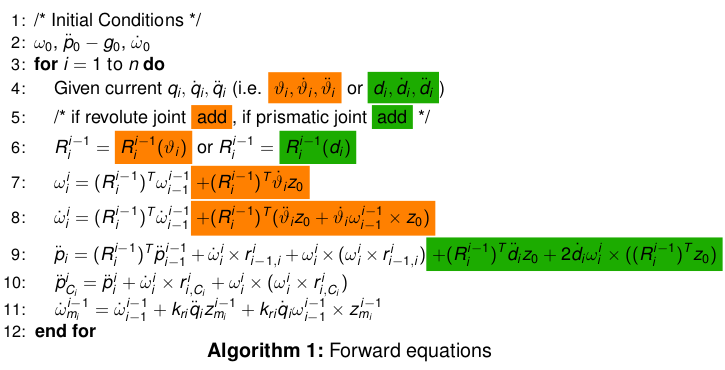
\includegraphics[keepaspectratio,width=0.6\textwidth]{rne_forw}
\end{figure}
\begin{figure}[h]
\centering
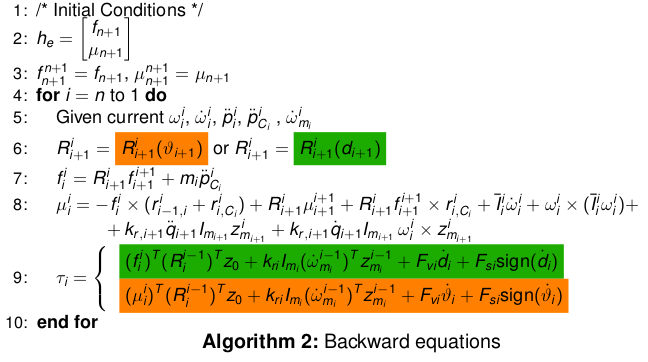
\includegraphics[keepaspectratio,width=0.6\textwidth]{rne_back}
\end{figure}

To check the results, the resulting $B_{RNE}$, $C_{RNE}$ e $g_{RNE}$ were compared to the corresponding quantities computed with the Lagrangian method, in a random robot configuration and joint velocities:

\begin{align*}
B_{RNE} = \begin{bmatrix}
 0.4372& -0.61966  & 0.03208\\
-0.6196&    1.549 &-0.06925\\
 0.03208& -0.069256  &0.04708
\end{bmatrix}&\;\;\;\;\; B_{L} = \begin{bmatrix}
 0.4372& -0.61966   &0.03208\\
-0.6196&    1.549& -0.06925\\
 0.03208& -0.069256 & 0.04708
\end{bmatrix}\\
C_{RNE} = \begin{bmatrix}
 -0.001341\\
0.0005088\\
 -4.893e-5
\end{bmatrix}&\;\;\;\;\; C_{L} = \begin{bmatrix}
 -0.001341\\
  -0.001073\\
0.0002748
\end{bmatrix}\\
g_{RNE} = \begin{bmatrix}
 0\\
  0\\
-0.5539
\end{bmatrix}&\;\;\;\;\; g_{L} = \begin{bmatrix}
0\\
 0\\
-0.5539
\end{bmatrix}\\
\end{align*}


\newpage

\section{Assignment 5}

\subsection{Compute the dynamic model in the operational space}

The dynamic model in the operational space is described as follows:

\begin{align*}
B_A(x)\ddot x+C_A(x,\dot x)\dot x+g_A(x)=u-u_e
\end{align*}
where:
\begin{align*}
B_A(x)&=J_A^{-T}BJ_A^{-1}\\
C_A\dot x &= (J_A^{-T}C-B_A\dot J_A)\dot q\\
g_A(x)&=J_A^{-T}g\\
u &= T_A^Th\\
u_e&=T_A^Th_e
\end{align*}

with:

\begin{equation*}
T_A=\begin{bmatrix}
1&0&0&0&0&0\\
0&1&0&0&0&0\\
0&0&1&0&0&0\\
0&0&0&0&C_1&0\\
0&0&0&0&S_1&0\\
0&0&0&1&0&0
\end{bmatrix}
\end{equation*}
\begin{equation*}\dot J_A = \begin{bmatrix}
C_1\dot q_2 - S_1\dot q_1(d_2 + q2) - a_1C_1\dot q_1 - a_3C_3S_1\dot q_1 - a_3C_1S_3\dot q_3& C_1\dot q_1& - a_3C_1S_3\dot q_1 - a_3C_3S_1\dot q_3\\
S_1\dot q_2 + C_1\dot q_1(d_2 + q2) - a_1S_1\dot q_1 + a_3C_1C_3\dot q_1 - a_3S_1S_3\dot q_3& S_1\dot q_1&   a_3C_1C_3\dot q_3 - a_3S_1S_3\dot q_1\\
0&                 0&  -a_3S_3\dot q_3\\
0&0&0\\0&0&0\\0&0&0
 \end{bmatrix}
\end{equation*}

The resulting matrices are not reported for space reasons.

\newpage

\section{Assignment 6}

\subsection{Design the joint space PD control law with gravity compensation}

The goal is to implement the following architecture:

\begin{figure}[h]
\centering
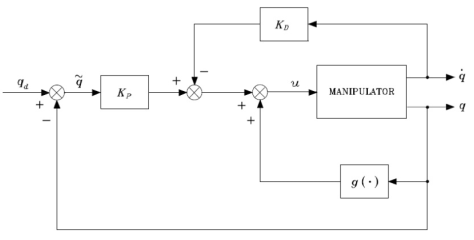
\includegraphics[keepaspectratio,width=0.4\textwidth]{joint_PD_arch}
\caption{Joint space PD control law with gravity compensation architecture}
\end{figure}

The architecture follows the control law:

\begin{equation*}
\tau = g(q) + K_P(q_d-q) + K_D(\dot q_d -q_d)\;\;\;\;\;\text{with }K_P = 50,K_D =  10
\end{equation*}

The architecture was implemented in SIMULINK as follows:

\begin{figure}[h]
\centering
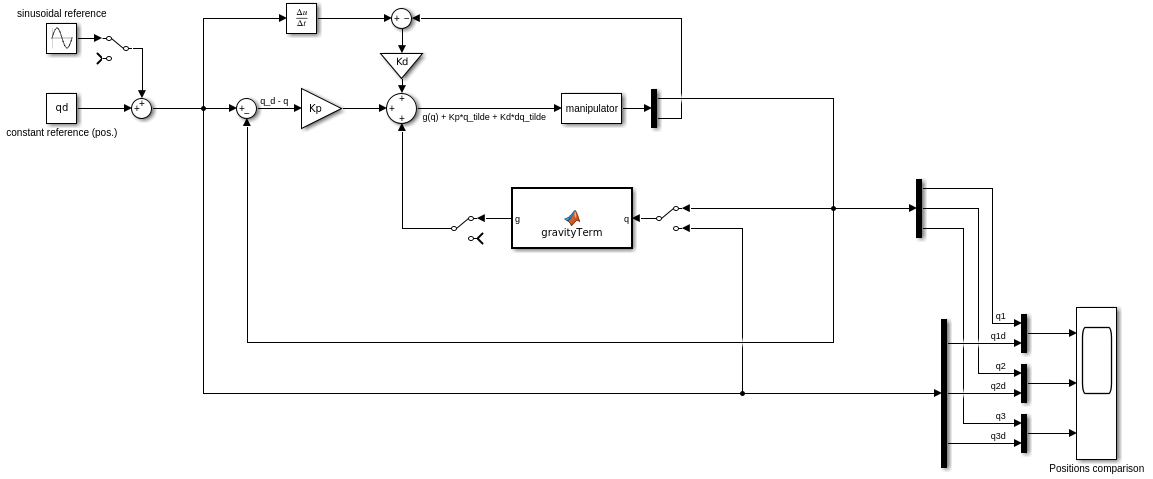
\includegraphics[keepaspectratio,width=0.6\textwidth]{joint_PD}
\caption{Joint space PD control law with gravity compensation SIMULINK model}
\end{figure}

\begin{figure}[H]
\centering
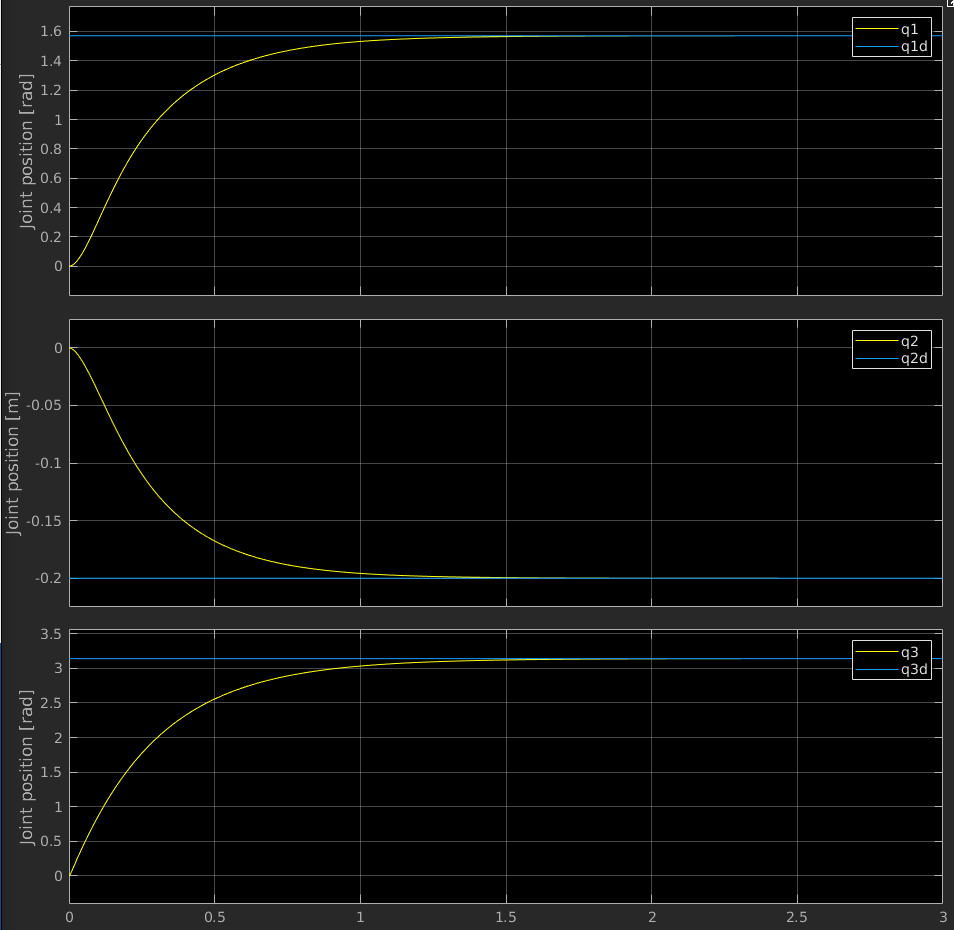
\includegraphics[keepaspectratio,width=0.5\textwidth]{joint_PD_correct}
\caption{Joint positions - constant reference $q_d=\begin{bmatrix}
\pi/2& -0.2& \pi\end{bmatrix}^T$}
\end{figure}

\subsection{What happens if g(q) is not taken into account?}

\begin{figure}[H]
\centering
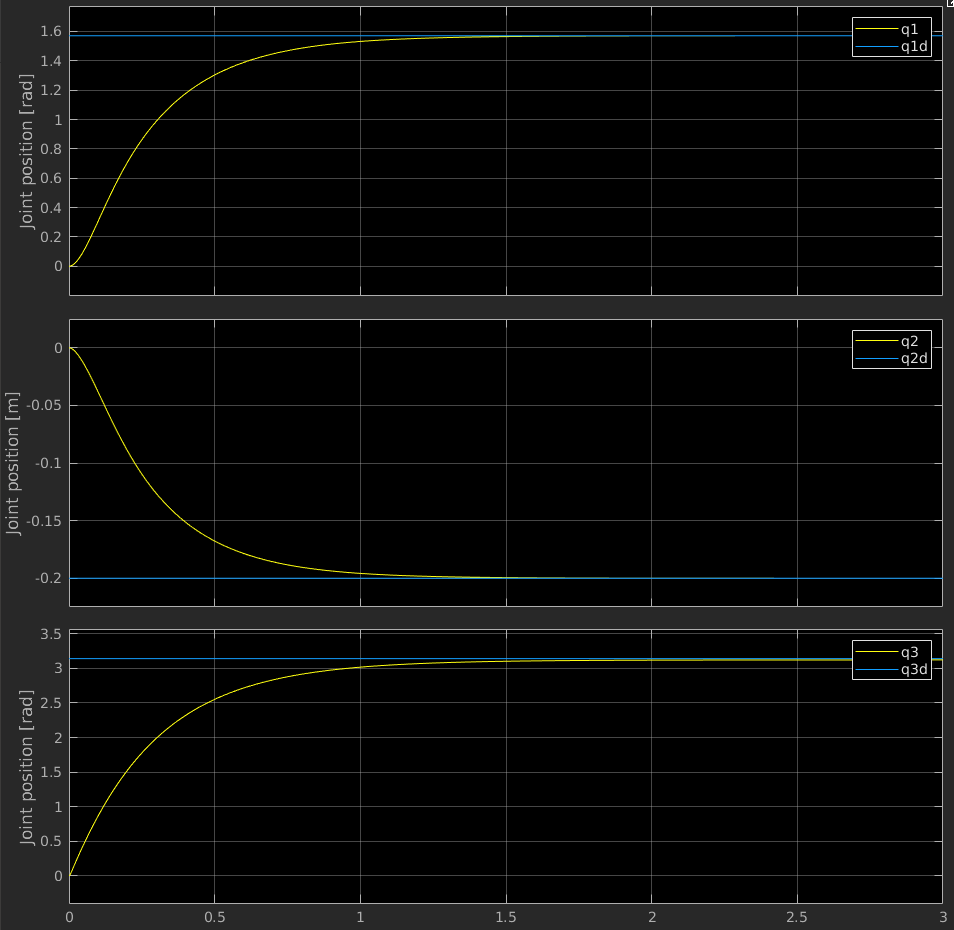
\includegraphics[keepaspectratio,width=0.6\textwidth]{joint_PD_nog}
\caption{Joint positions - $g(q)=0$}
\end{figure}

\subsection{What happens if the gravity term is equal to g($q_d$)?}


\begin{figure}[H]
\centering
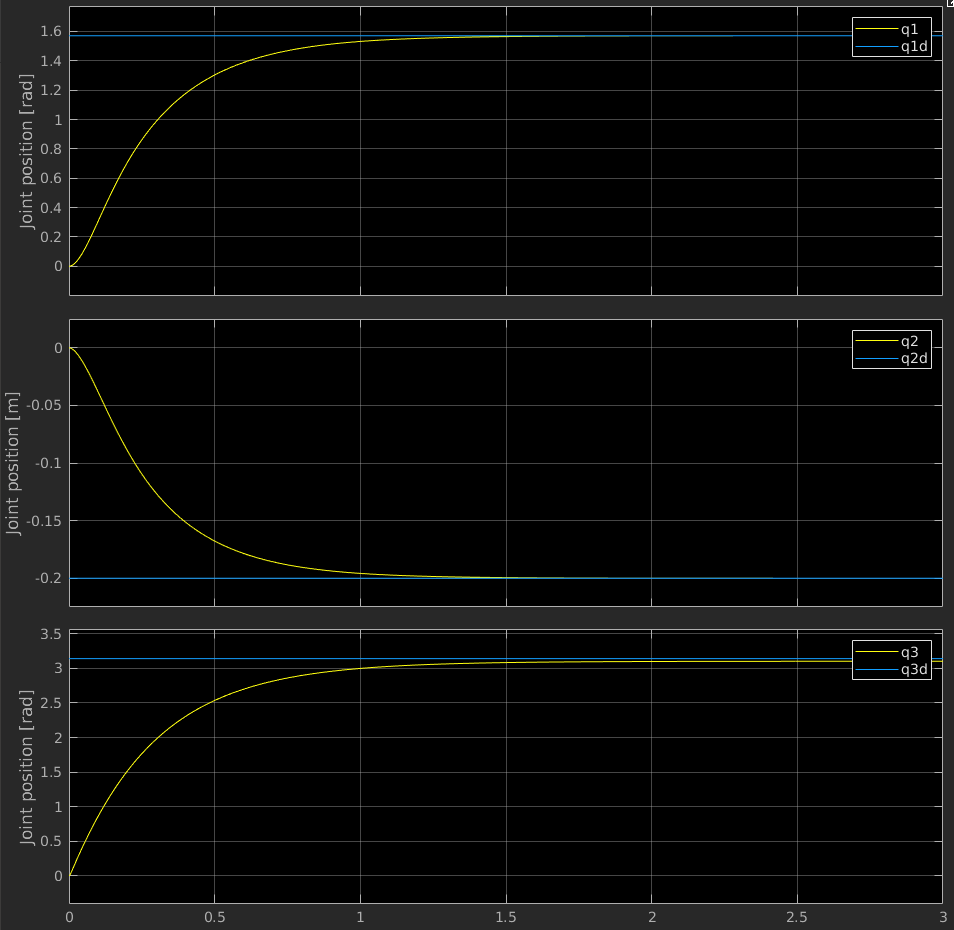
\includegraphics[keepaspectratio,width=0.6\textwidth]{joint_PD_wrongg}
\caption{Joint positions - $g(q)=g(q_d)$}
\end{figure}

\subsection{What happens if $q_d$ is not constant?}


\begin{figure}[H]
\centering
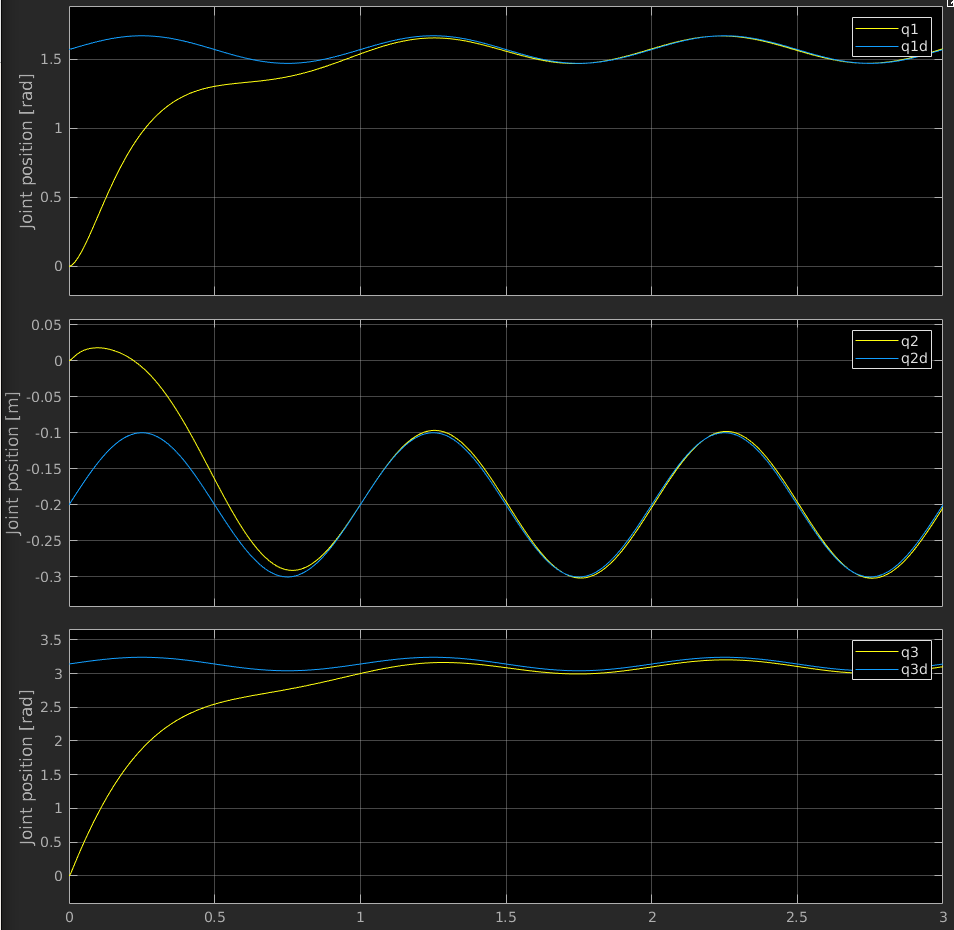
\includegraphics[keepaspectratio,width=0.6\textwidth]{joint_PD_sin}
\caption{Joint positions - sinusoidal reference $q_d = \begin{bmatrix}
\pi/2& -0.2& \pi
\end{bmatrix}^T + 0.1sin(2\pi)$}
\end{figure}


\newpage

\section{Assignment 7}

\subsection{Design the joint space inverse dynamics control law}

The goal is to implement the following architecture:

\begin{figure}[h]
\centering
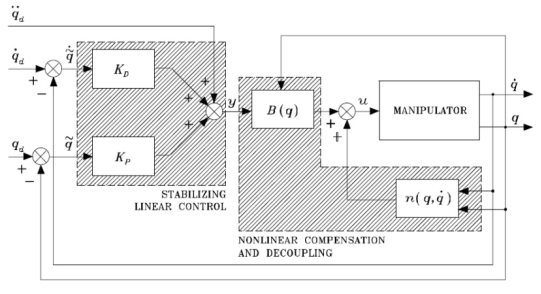
\includegraphics[keepaspectratio,width=0.4\textwidth]{inv_dyn_arch}
\caption{Joint space PD control law with gravity compensation architecture}
\end{figure}

The architecture works by linearizing non-linear dynamics and by decoupling each joint variable. It does so by implementing an inner feedback loop:

\begin{equation*}
\tau = B(q)y+n(q,\dot q)
\end{equation*}

where $n(q,\dot q) = C(q,\dot q)\dot q+g(q)$ and $y$ is controlled by the outer feedback loop:

\begin{equation*}
y = \ddot q_d+K_D(\dot q_d-q)+K_P(q_d-q)\;\;\;\;\text{with }K_P=50,K_D=10
\end{equation*}

The architecture was implemented in SIMULINK as follows:

\begin{figure}[h]
\centering
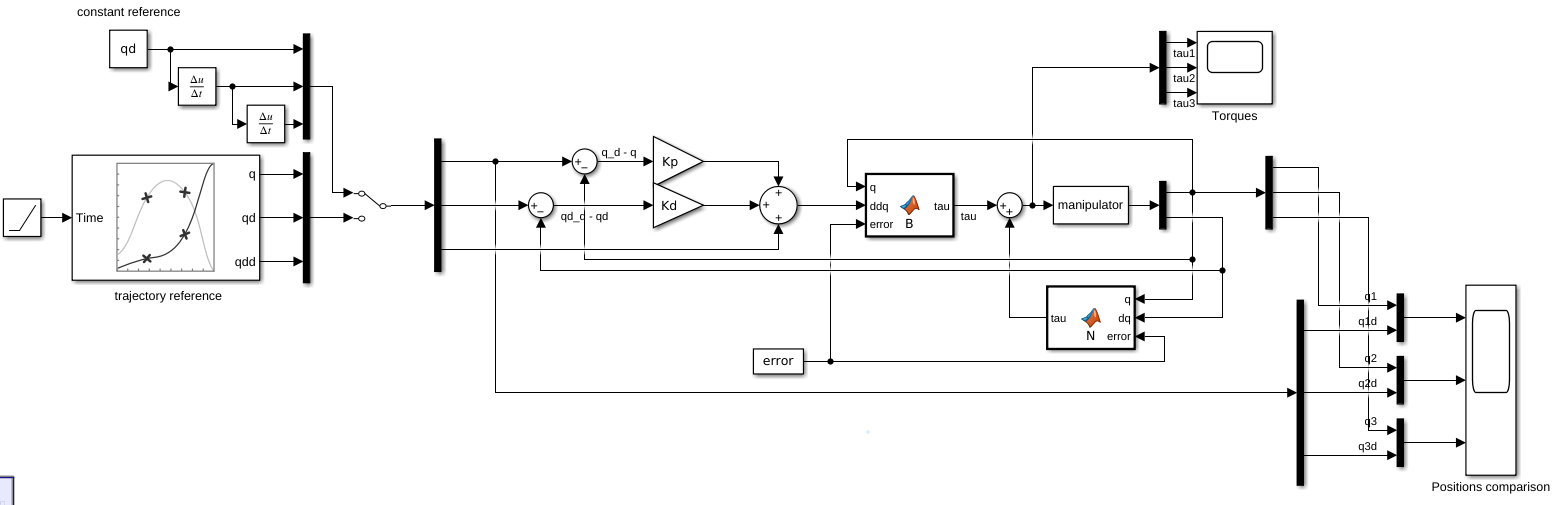
\includegraphics[keepaspectratio,width=0.8\textwidth]{inv_sim}
\caption{Joint space inverse control law SIMULINK model}
\end{figure}

The architecture is tested with a quintic polynomial trajectory that passes through the waypoints:

\begin{align*}
q_{d}\mid_{t=0.5} &= \begin{bmatrix}
\pi/3 & -0.2 & \pi/3
\end{bmatrix}\\
q_{d}\mid_{t=1} &= \begin{bmatrix}
-\pi/3 & -0.1 & \pi/4
\end{bmatrix}\\
q_{d}\mid_{t=1.5} &= \begin{bmatrix}
0 & -0.2 & 0
\end{bmatrix}\\
q_{d}\mid_{t=2} &= \begin{bmatrix}
\pi/2 & 0 & -\pi/4
\end{bmatrix}\\
q_{d}\mid_{t=2.5} &= \begin{bmatrix}
\pi/3 & -0.1 & \pi/4
\end{bmatrix}\\
q_{d}\mid_{t=3} &= \begin{bmatrix}
0 & 0 & 0
\end{bmatrix}
\end{align*}

The boundary conditions for the generation of the quintic trajectory are that the velocity and acceleration are null in each of the waypoints.

To show the effect of decoupling, the architecture was also tested against a constant reference $q_d=\begin{bmatrix}
\pi/1& -0.2&\pi
\end{bmatrix}$.

\begin{figure}[H]
\begin{minipage}{0.5\textwidth}
\centering
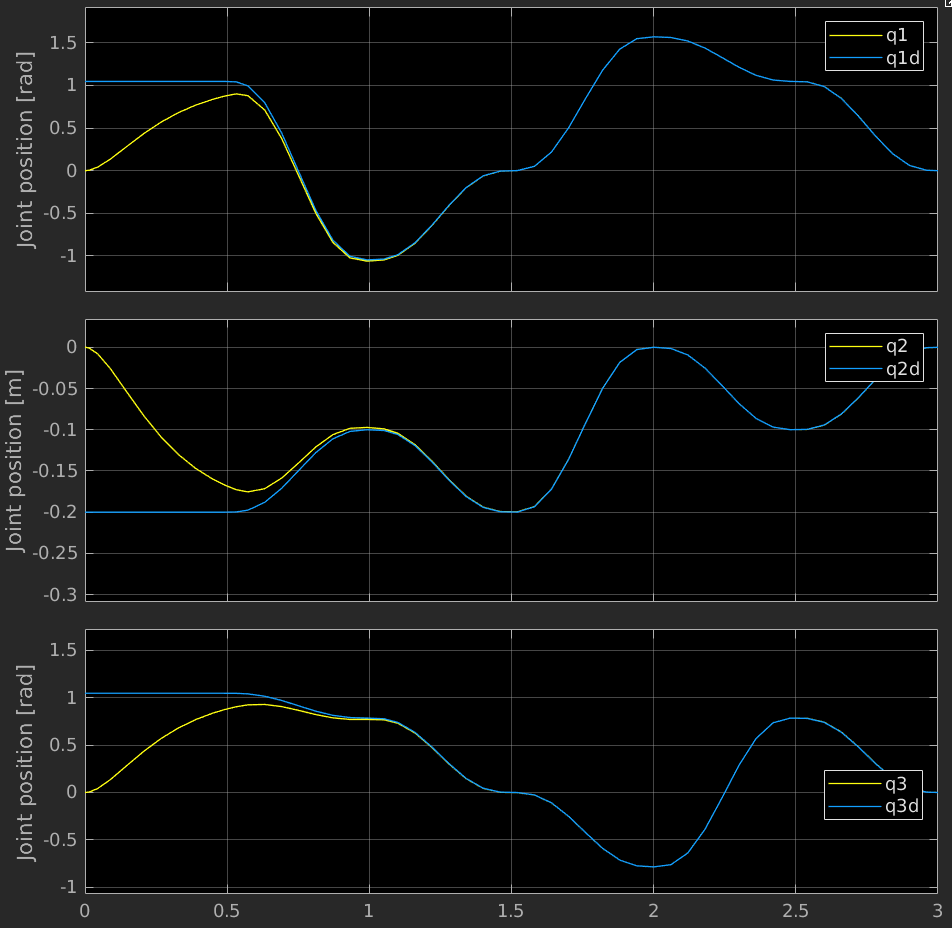
\includegraphics[keepaspectratio,width=\textwidth]{inv_correct}
\caption{Joint positions}
\end{minipage}
\begin{minipage}{0.5\textwidth}
\centering
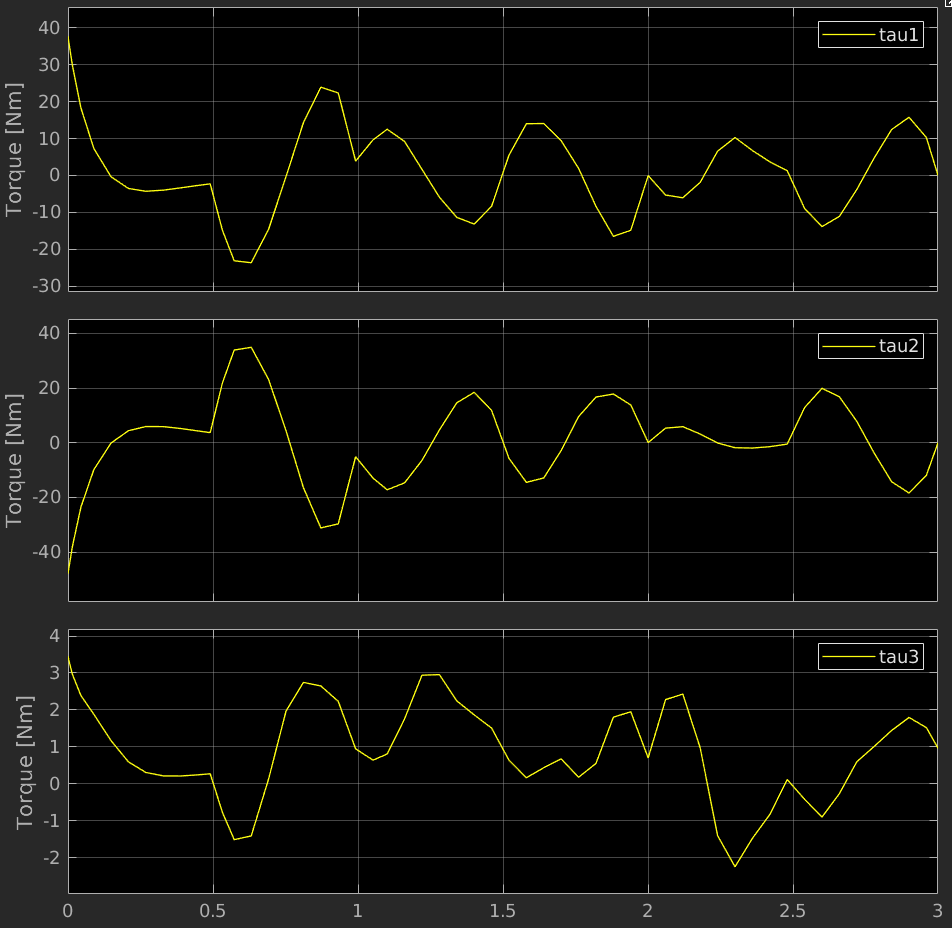
\includegraphics[keepaspectratio,width=\textwidth]{inv_correct_torque	}
\caption{Joint torques}
\end{minipage}
\end{figure}

\begin{figure}[H]
\centering
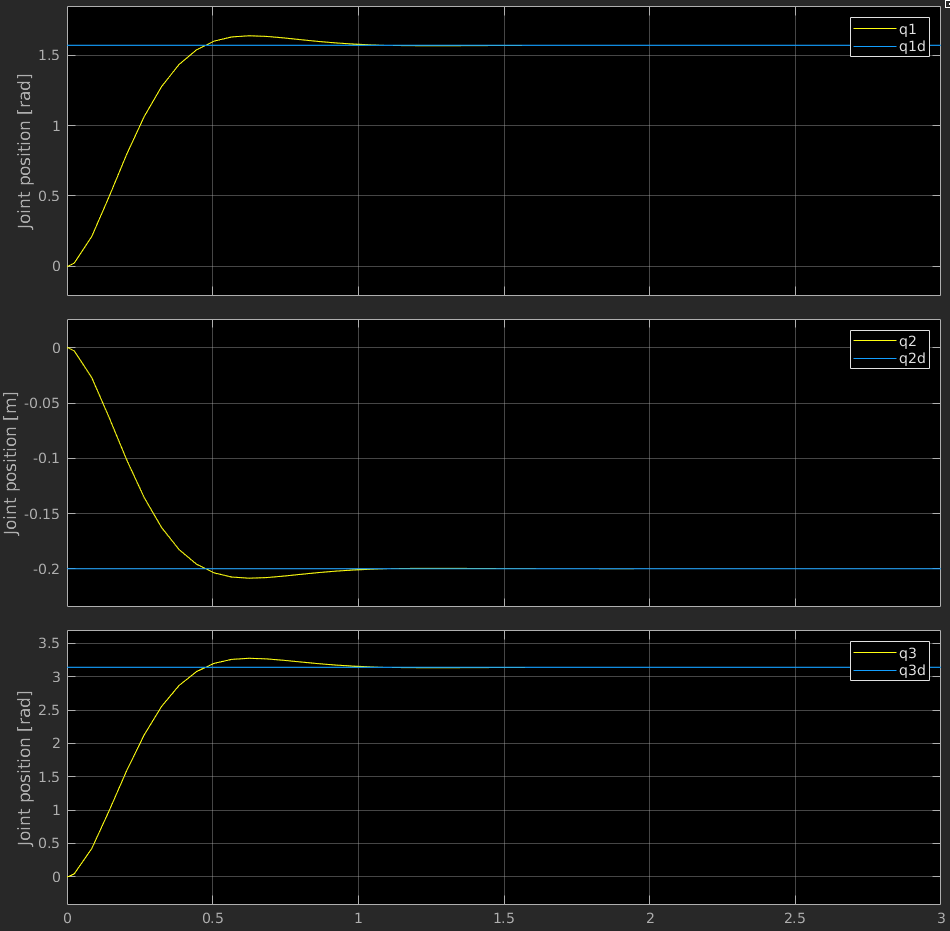
\includegraphics[keepaspectratio,width=0.65\textwidth]{inv_same_beh}
\caption{Joint positions - constant reference, decoupling}
\end{figure}

\subsection{Check the behaviour of the control law when the B, C and g values are different than the true ones}

\begin{figure}[H]
\centering
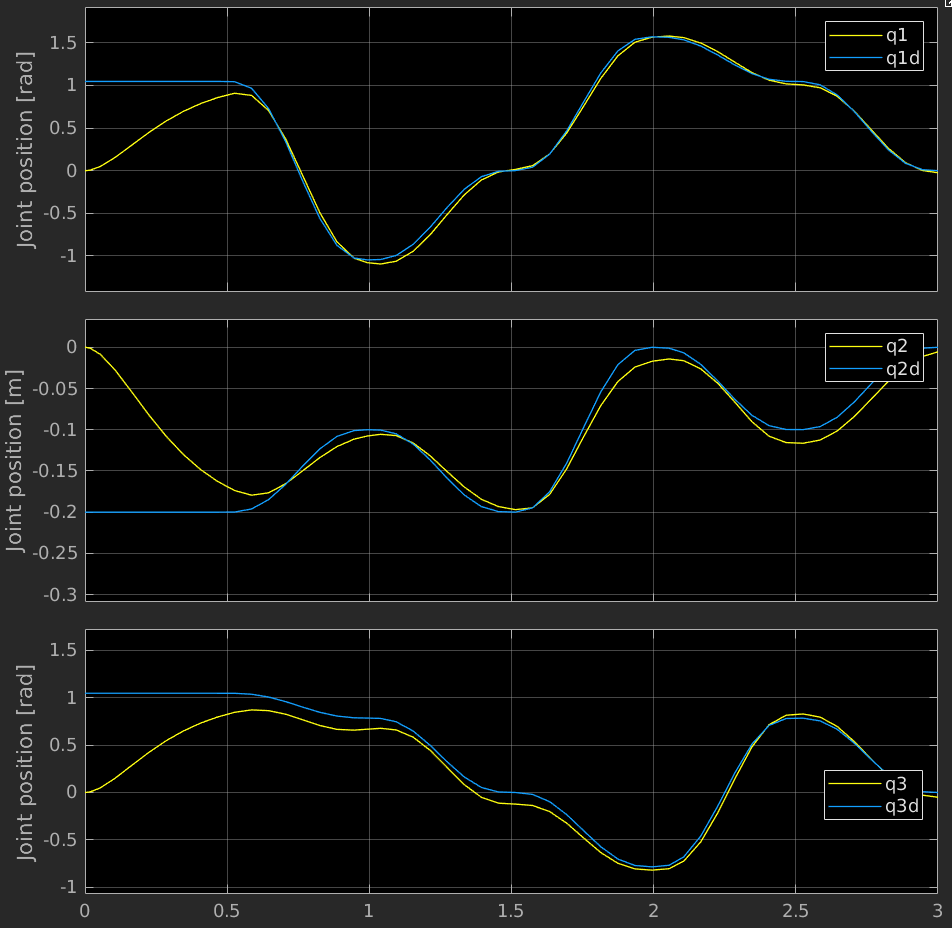
\includegraphics[keepaspectratio,width=0.65\textwidth]{inv_wrongB}
\caption{Joint positions - changed values of the link masses}
\end{figure}

\subsection{What happens to the torque values when the settling time of the equivalent second order systems is chosen very small?}

\begin{figure}[H]
\centering
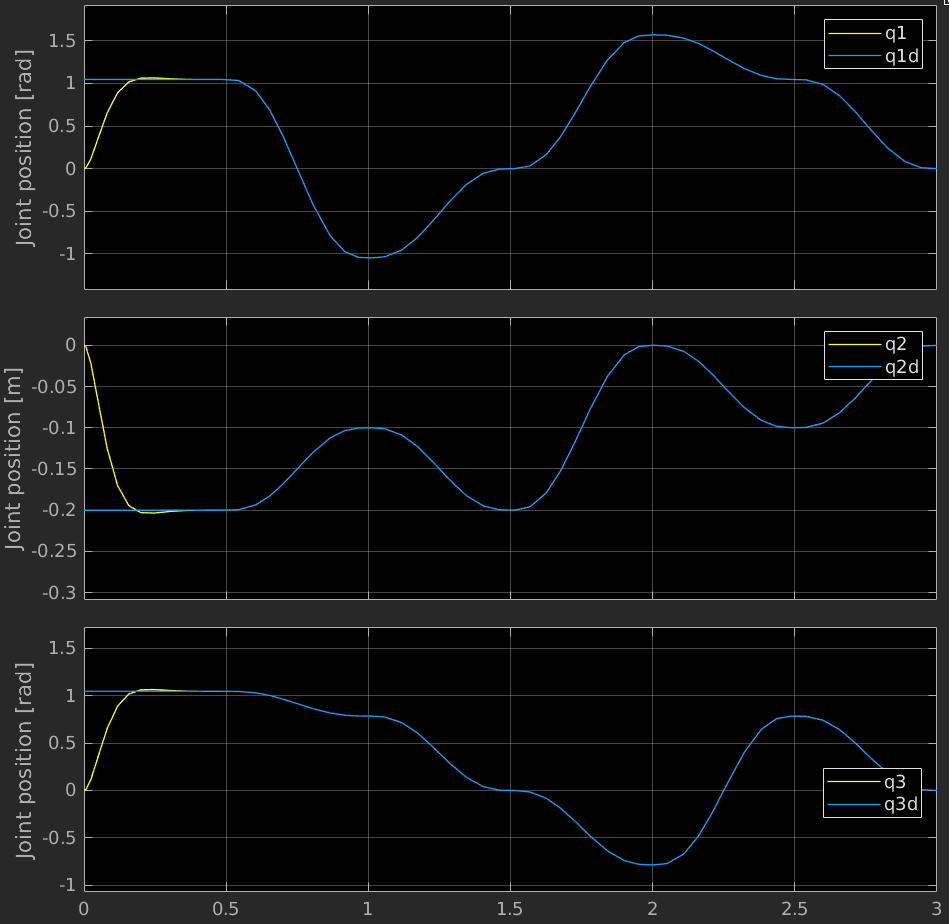
\includegraphics[keepaspectratio,width=0.6\textwidth]{inv_small_rising}
\caption{Joint positions - $K_P=500,K_D=35$}
\end{figure}
\begin{figure}[H]
\centering
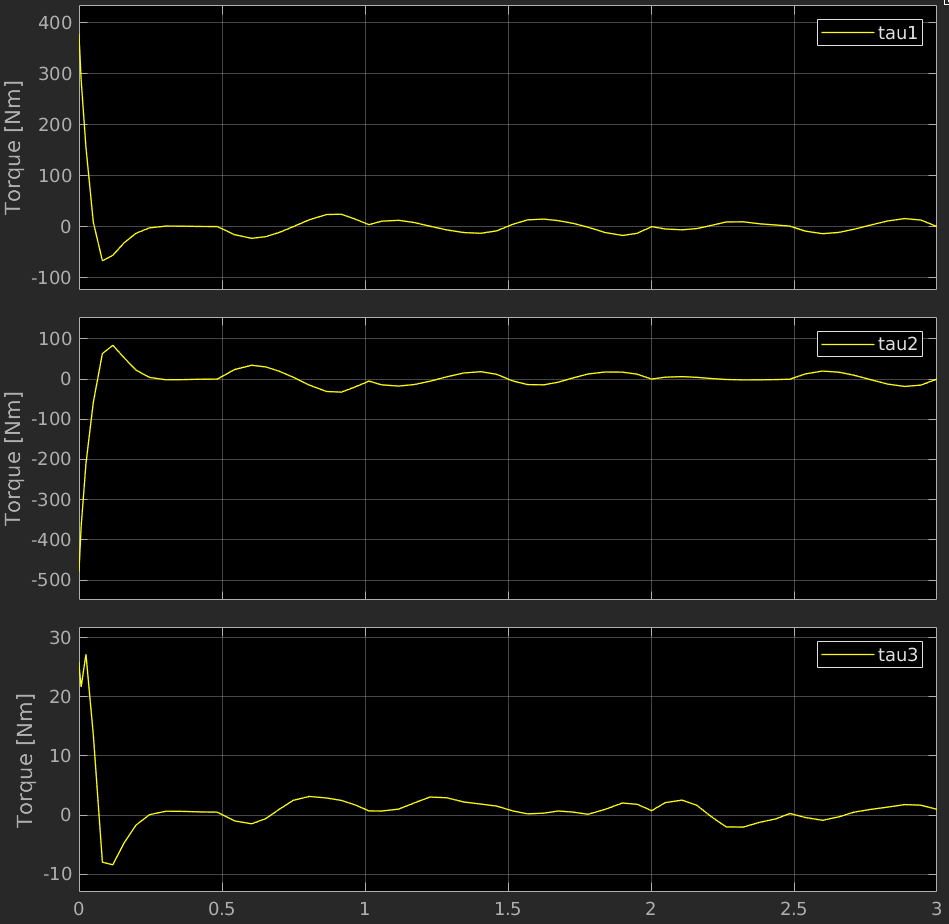
\includegraphics[keepaspectratio,width=0.6\textwidth]{inv_small_rising_torque}
\caption{Joint torques - $K_P=500,K_D=35$}
\end{figure}

\newpage

\section{Assignment 8}

\subsection{Implement in Simulink the Adaptive Control law for the a 1-DoF link under gravity.}

\begin{figure}[H]
\centering
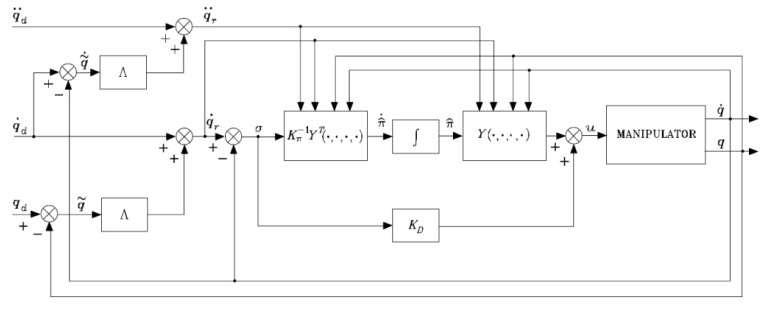
\includegraphics[keepaspectratio,width=0.6\textwidth]{adaptive_arch}
\caption{Adaptive control architecture}
\end{figure}

The adaptive control law tackles the problem of model uncertainty by implementing an on-line estimator of the robot's dynamic parameters. 

The plant is modelled with three dynamic parameters (inertia, friction and gravity term):

\begin{equation*}
I\ddot q + F\dot q + G\sin q = \tau\implies \tau = \begin{bmatrix}
\ddot q & \dot q & \sin q
\end{bmatrix}\begin{bmatrix}
I\\ F\\ G
\end{bmatrix}=Y(q,\dot q,\ddot q)\Theta
\end{equation*}

The estimation of the dynamic parameters is as follows:

\begin{equation*}
\hat\Theta=\begin{bmatrix}
\hat I\\\hat F\\\hat G
\end{bmatrix}=\begin{bmatrix}
\gamma_1 & 0 & 0\\ 0 & \gamma_2 & 0\\ 0 & 0 & \gamma_3
\end{bmatrix}\begin{bmatrix}
\ddot q\\\dot q\\\sin q
\end{bmatrix}(\dot q_r-\dot q)
\end{equation*}

where the reference velocity is computed as:

\begin{equation*}
\dot q_r = \dot q_d+\lambda (q_d-q) = \dot q_d+\frac{K_P}{K_D} (q_d-q)
\end{equation*}

The architecture is implemented in SIMULINK as follows:

\begin{figure}[H]
\centering
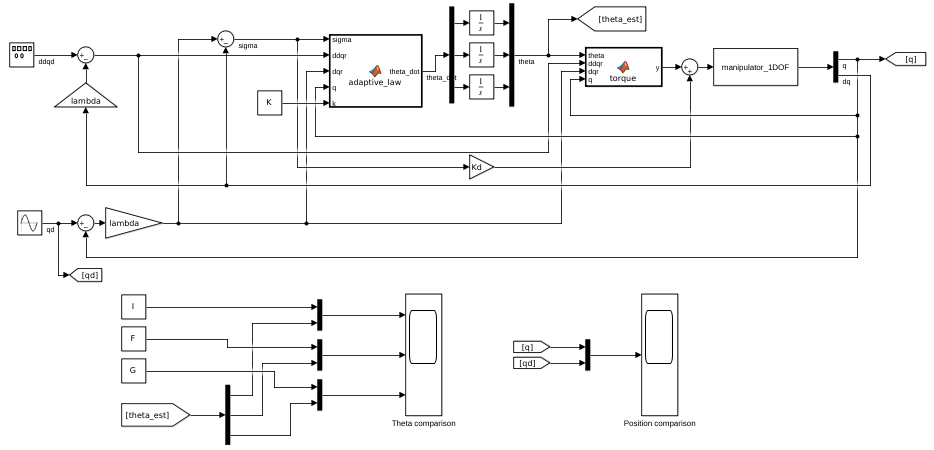
\includegraphics[keepaspectratio,width=0.6\textwidth]{adaptive_sim}
\caption{Adaptive control SIMULINK model}
\end{figure}

The model is tested with a sinusoidal reference trajectory $q_d=A\sin(\omega t)$ and a periodic square wave acceleration reference $\ddot q_d = square(\pm A)$, with $A=1$ and $\omega = 2\pi$.

\newpage

\begin{figure}[H]
\centering
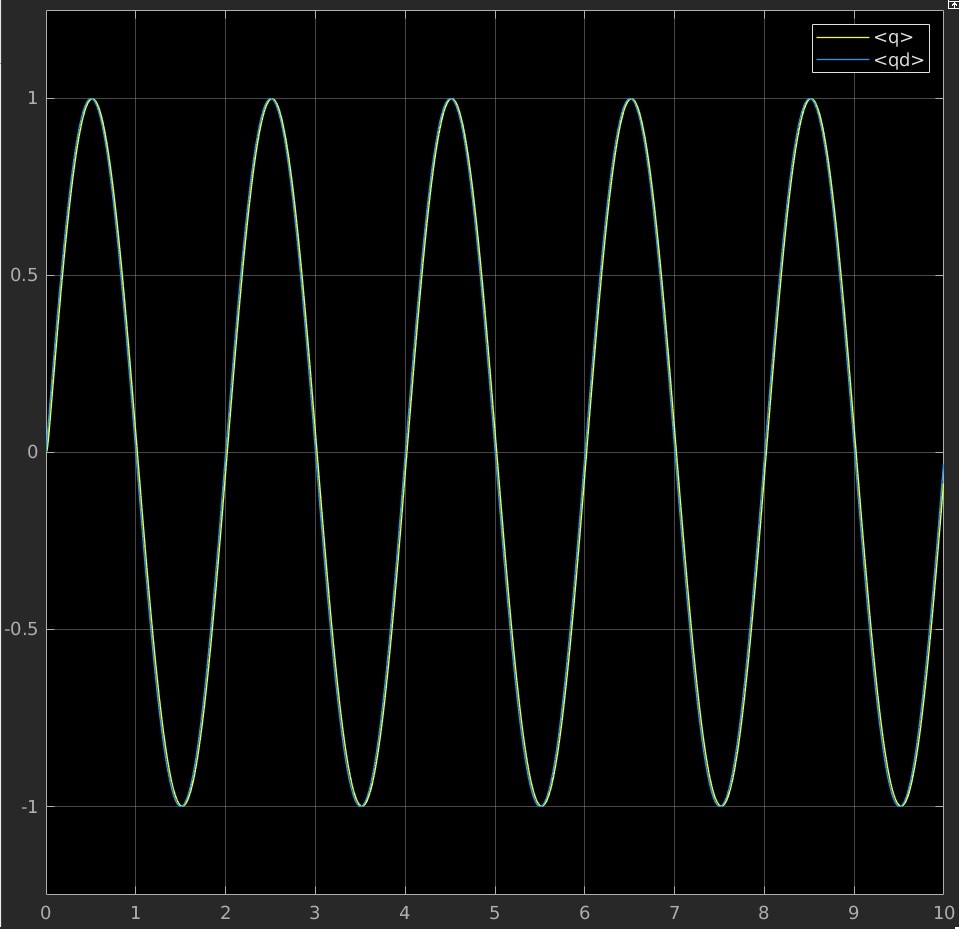
\includegraphics[keepaspectratio,width=0.6\textwidth]{adaptive_pos}
\caption{Adaptive control - position reference tracking}
\end{figure}

\begin{figure}[H]
\centering
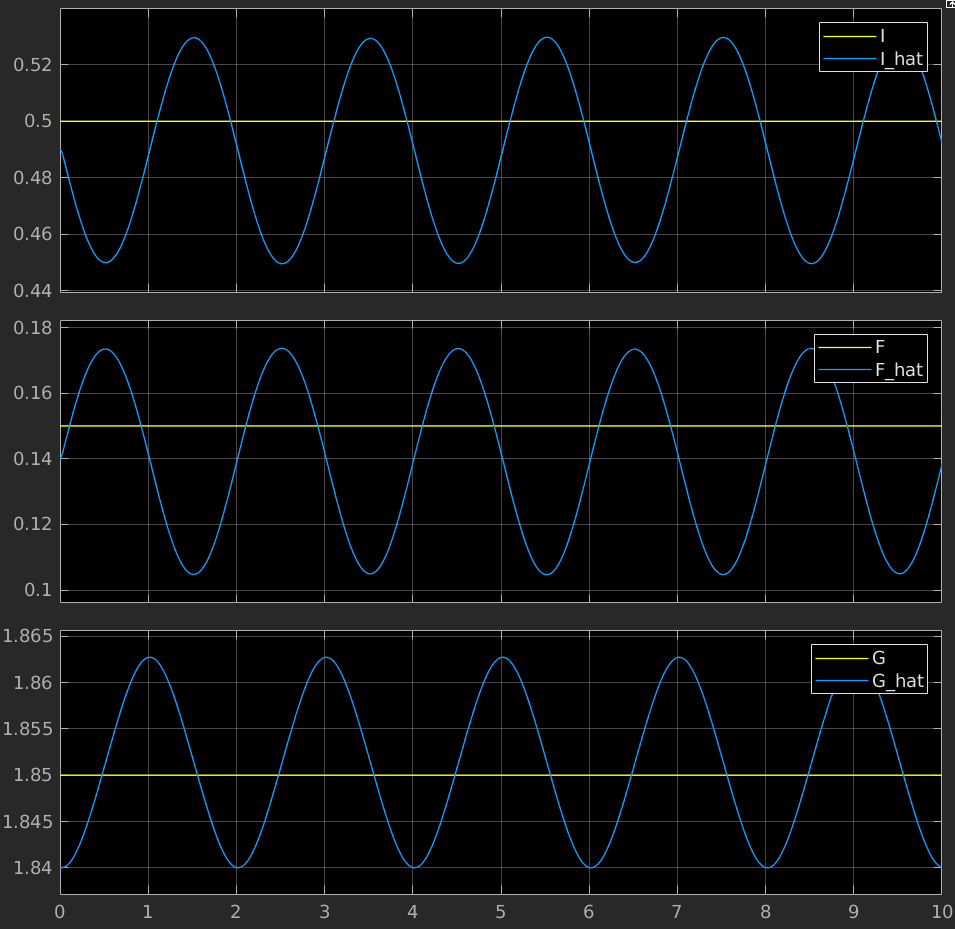
\includegraphics[keepaspectratio,width=0.6\textwidth]{adaptive_theta}
\caption{Adaptive control - parameter estimation}
\end{figure}


\newpage

\section{Assignment 9}

\subsection{Design the operational space PD control law with gravity compensation}

\begin{figure}[H]
\centering
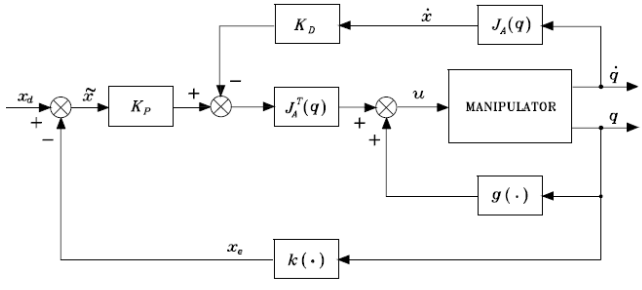
\includegraphics[keepaspectratio,width=0.4\textwidth]{op_pd_arch}
\caption{Operational space PD control law with gravity compensation architecture}
\end{figure}

The operational space PD control law with gravity compensation works exactly the same as the joint space one, except for the transformation of the joint space quantities into the corresponding operational space ones with direct kinematics (i.e. with the use of the transformation matrix $T$ and of the analytical Jacobian $JA$). The control law parameters are $K_P=50,K_D=10$. The architecture was tested with a constant pose reference obtained by applying direct kinematics to the joint configuration $q=\begin{bmatrix}
-\pi/3&-0.1&\pi/2
\end{bmatrix}$.

\begin{figure}[H]
\centering
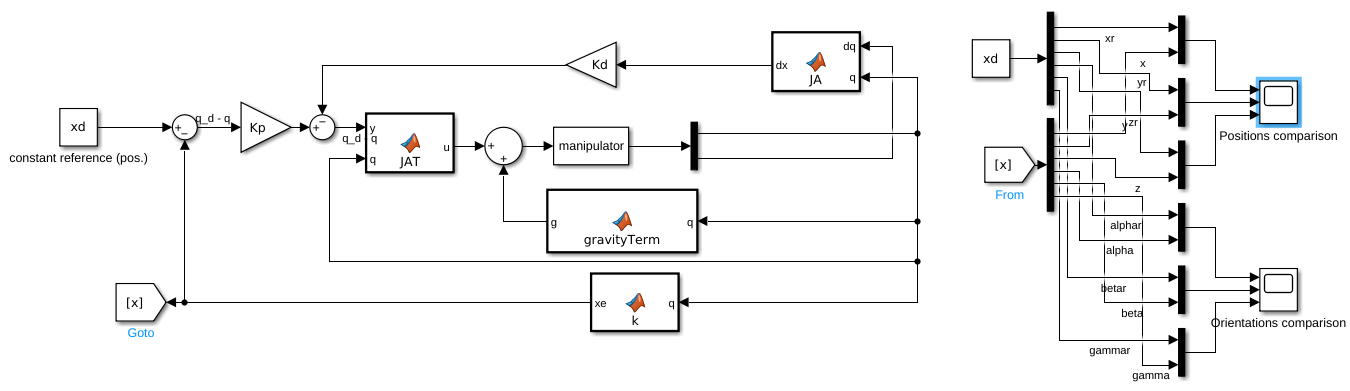
\includegraphics[keepaspectratio,width=0.7\textwidth]{op_pd_sim}
\caption{Operational space PD control law with gravity compensation SIMULINK model}
\end{figure}

\begin{figure}[H]
\begin{minipage}{0.5\textwidth}
\centering
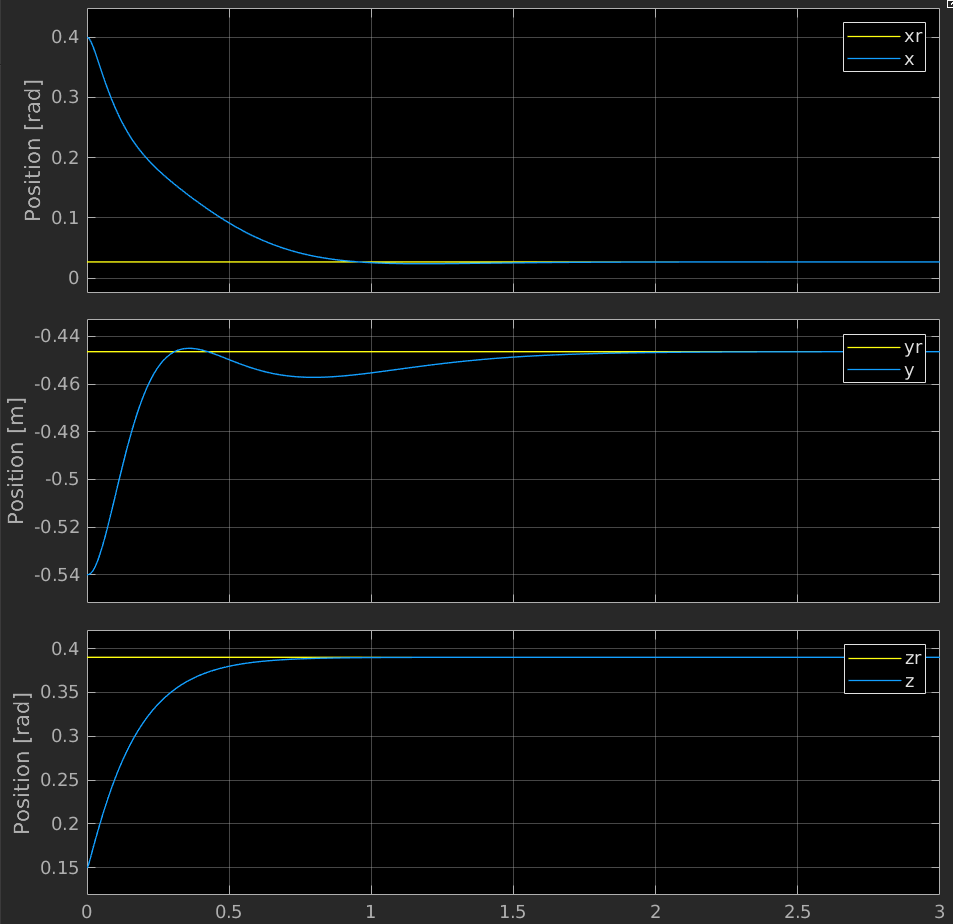
\includegraphics[keepaspectratio,width=\textwidth]{op_pd_pos}
\caption{Pose tracking - end-effector xyz coordinates}
\end{minipage}
\begin{minipage}{0.5\textwidth}
\centering
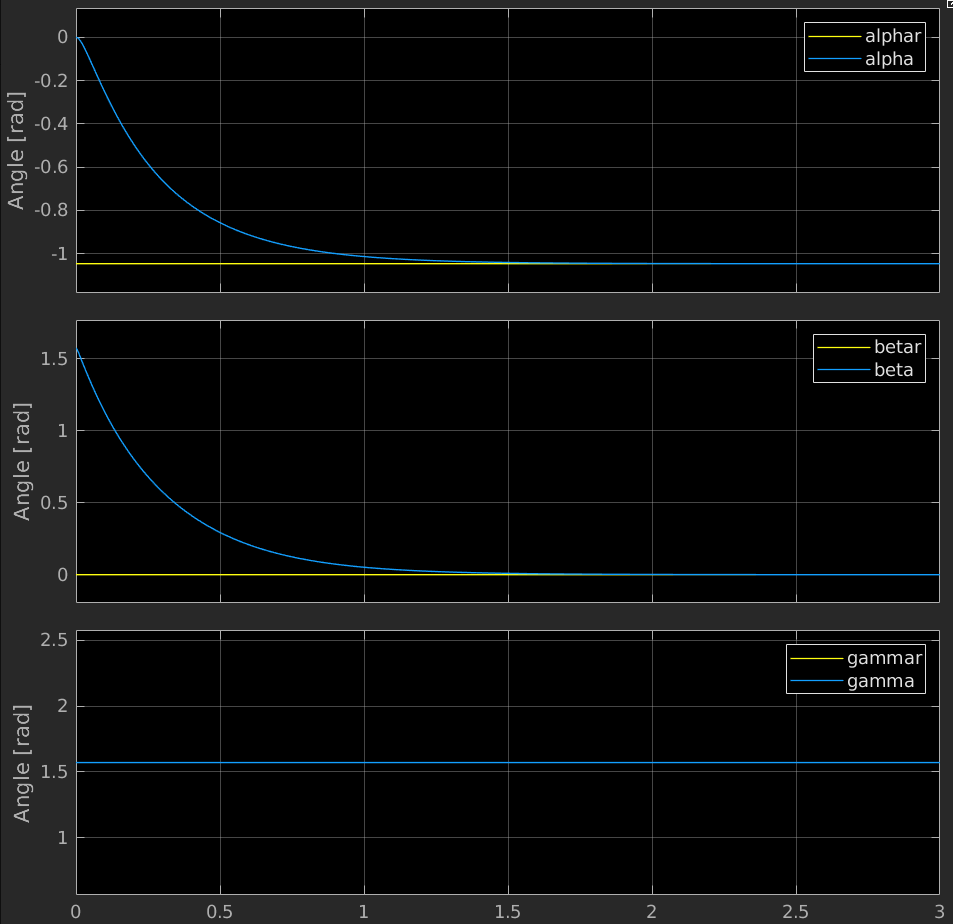
\includegraphics[keepaspectratio,width=\textwidth]{op_pd_or}
\caption{Pose tracking - end-effector $\alpha\beta\gamma$ coordinates}
\end{minipage}
\end{figure}

\newpage

\section{Assignment 10}

\subsection{Design the operational space inverse dynamics control law}

\begin{figure}[H]
\centering
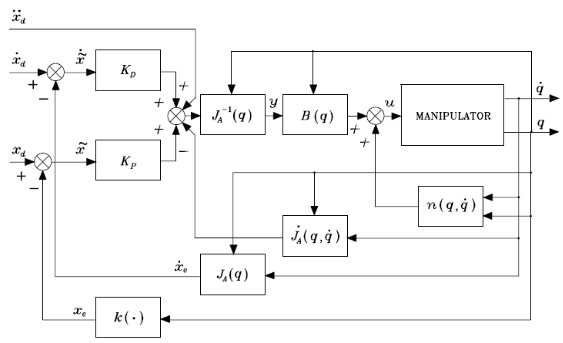
\includegraphics[keepaspectratio,width=0.35\textwidth]{op_inv_arch}
\caption{Operational space inverse dynamics control law architecture}
\end{figure}

The operational space inverse dynamics control law works exactly the same as the joint space one, except for the transformation of the joint space quantities into the corresponding operational space ones with direct kinematics (i.e. with the use of the transformation matrix $T$, the analytical Jacobian $JA$ and its inverse $JA^{-1}$ and derivative $\dot JA$). The control law parameters are $K_P=100,K_D=15$. The architecture was tested with a constant pose reference obtained by applying direct kinematics to the same waypoints seen in the joint space case.

\begin{figure}[H]
\centering
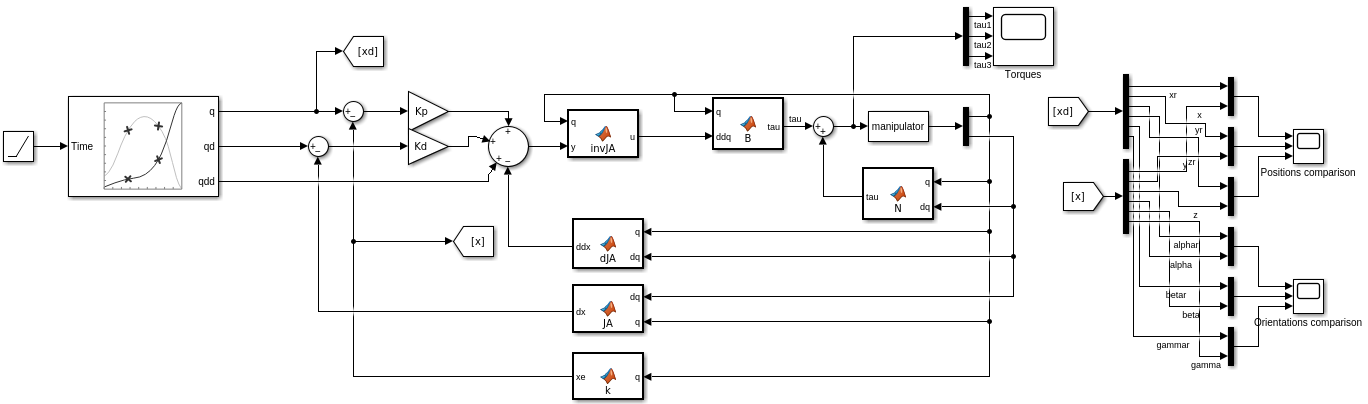
\includegraphics[keepaspectratio,width=0.7\textwidth]{op_inv_sim}
\caption{Operational space inverse dynamics control lawSIMULINK model}
\end{figure}

\begin{figure}[H]
\begin{minipage}{0.5\textwidth}
\centering
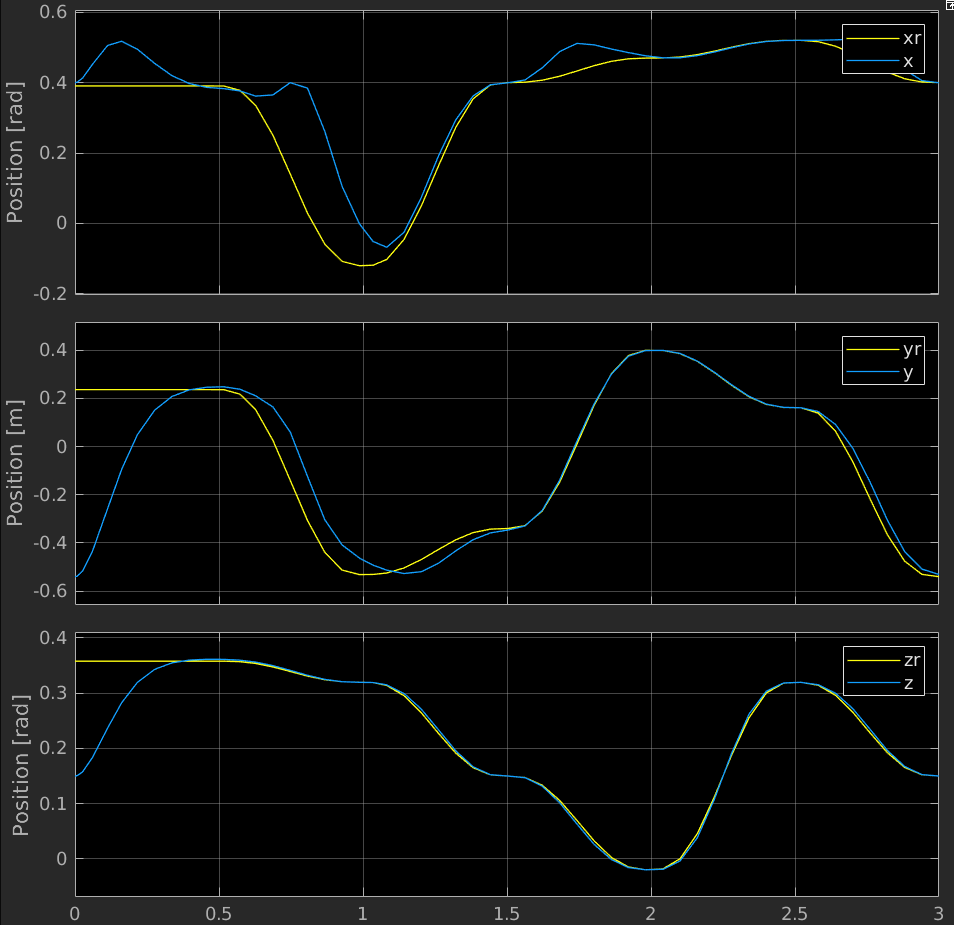
\includegraphics[keepaspectratio,width=\textwidth]{op_inv_pos}
\caption{Pose tracking - end-effector xyz coordinates}
\end{minipage}
\begin{minipage}{0.5\textwidth}
\centering
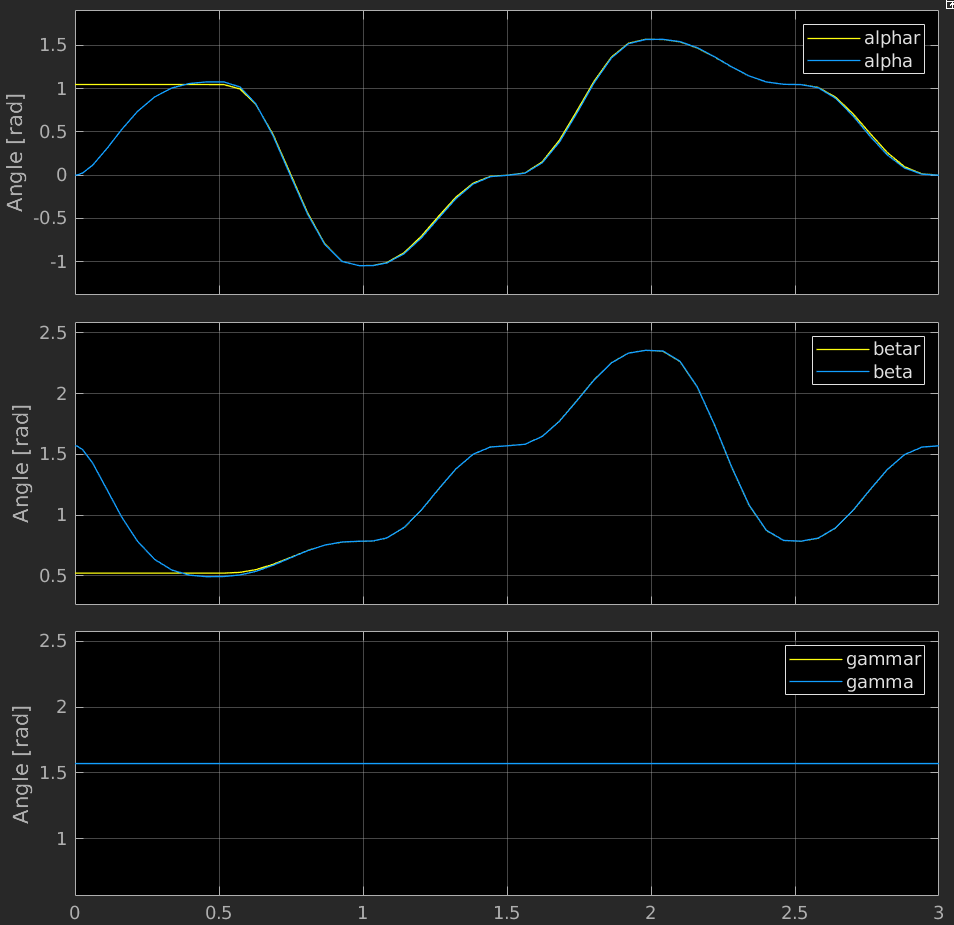
\includegraphics[keepaspectratio,width=\textwidth]{op_inv_or}
\caption{Pose tracking - end-effector $\alpha\beta\gamma$ coordinates}
\end{minipage}
\end{figure}

\newpage

\section{Assignment 11}

\subsection{Study the compliance control. Simulate the two “extreme” cases when the end-effector is interacting with the environment (considered as a planar surface)}

Compliance control is a form of indirect force control, i.e. a motion control without the explicit closure of a force feedback loop. Such an architecture allows the handling of non-null external wrenches $h_e$:

\begin{equation*}
B(q)\ddot q + C(q,\dot q)\dot q + g(q) = \tau -J^T(q)h_e
\end{equation*}

By looking at the above expression at the equilibrium we can relate the external wrench to the position error $\tilde x$ in operational space, through the use of the vector of external forces in operational space $h_A$ and a compliance matrix $K^{-1}$:

\begin{equation*}
\tilde x = K^{-1}h_A
\end{equation*}
The new PD control law becomes:

\begin{equation*}
\tau = g(q) + J_{Ad}^T(q,\tilde x)(K_P\tilde x-K_DJ_{Ad}(q,\tilde x)\dot q)\;\;\;\;\;\text{with }K_P=50,K_D=10
\end{equation*}

The architecture is modelled in SIMULINK as follows:

\begin{figure}[H]
\centering
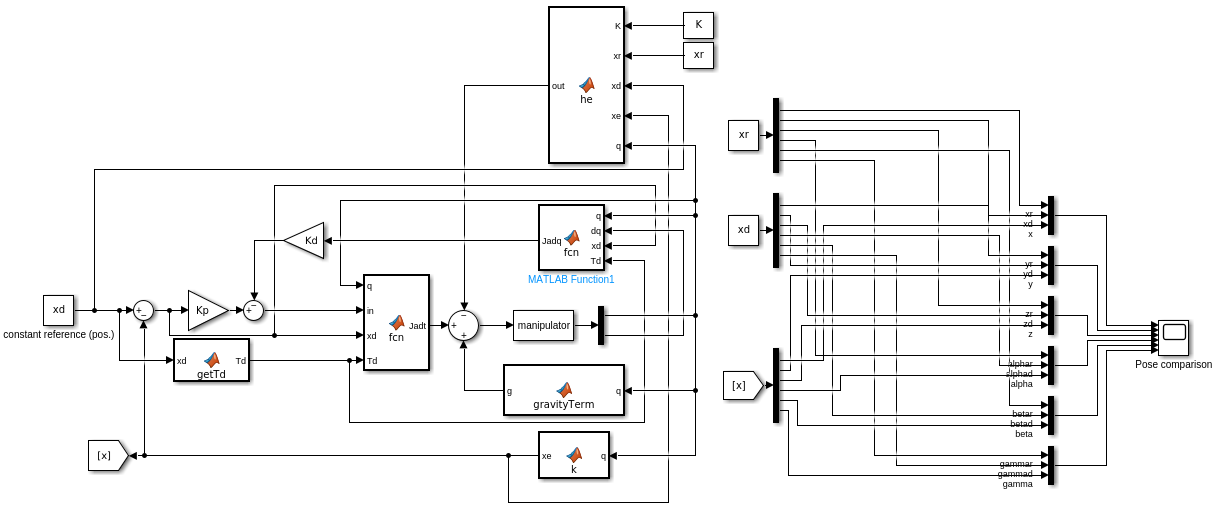
\includegraphics[keepaspectratio,width=\textwidth]{compliance_sim}
\caption{Compliance control in operational space SIMULINK model}
\end{figure}

To test the architecture, the manipulator was moved to $x_0=k(\begin{bmatrix}
0&-0.3&0
\end{bmatrix})$, with a desired position of $x_d=k(\begin{bmatrix}
0&-0.2&0
\end{bmatrix})$ and the environment placed at $x_e=k(\begin{bmatrix}
0&-0.1&0
\end{bmatrix})$. This was done to simplify the architecture, allowing for contact only in the $y$ direction.

\newpage

\subsection{$K_{env}\ll K_P$}

\begin{figure}[H]
\centering
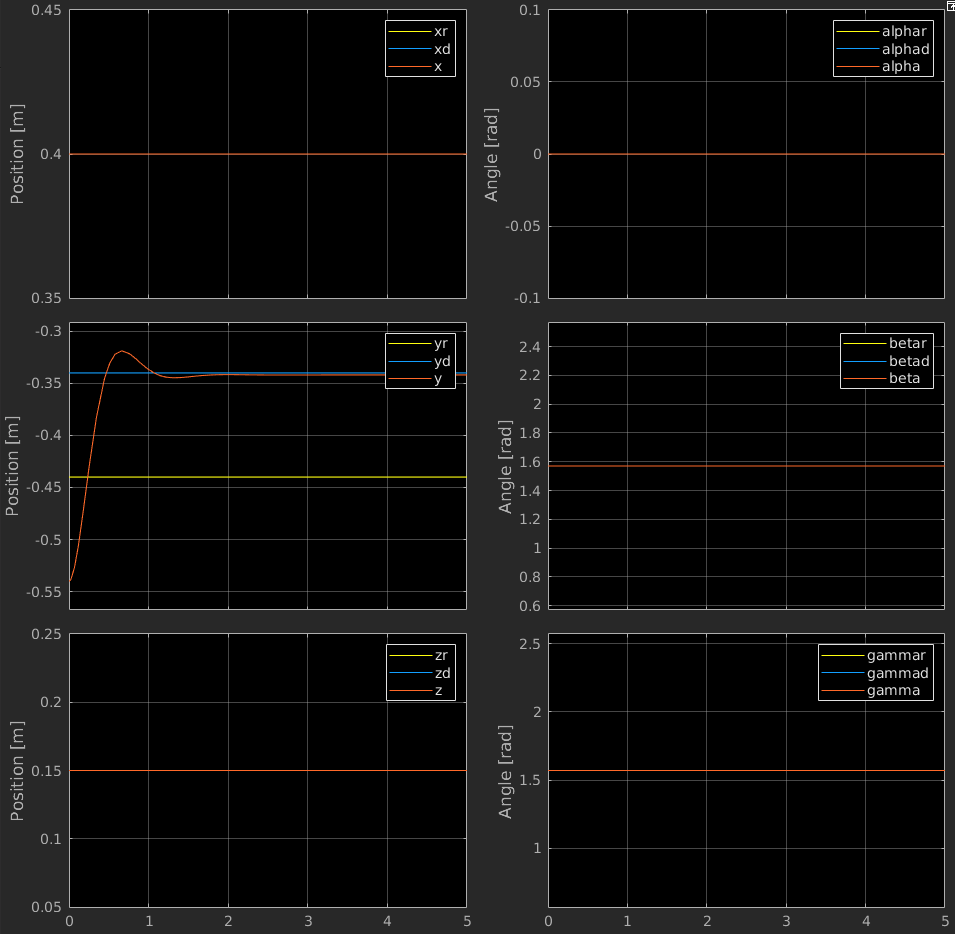
\includegraphics[keepaspectratio,width=\textwidth]{compliance_1}
\caption{Compliance control - $K=1$}
\end{figure}


\subsection{$K_{env}= K_P$}

\begin{figure}[H]
\centering
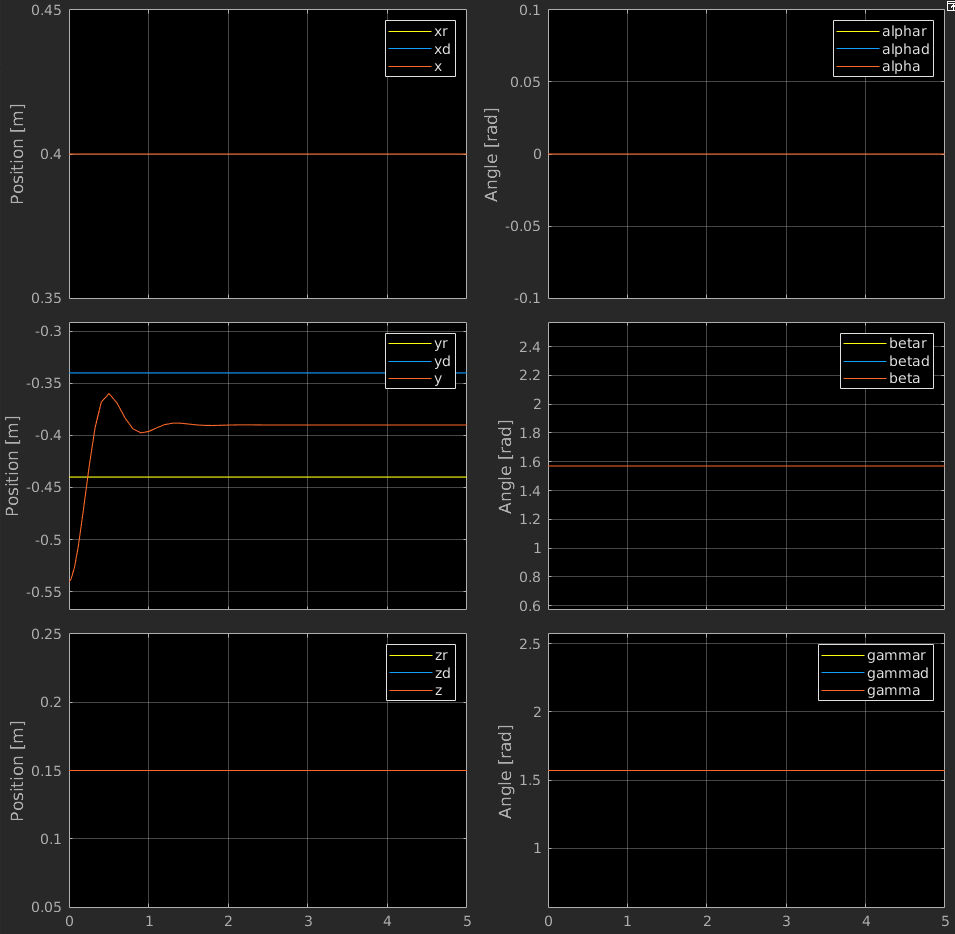
\includegraphics[keepaspectratio,width=\textwidth]{compliance_50}
\caption{Compliance control - $K=50$}
\end{figure}


\subsection{$K_{env}\gg K_P$}

\begin{figure}[H]
\centering
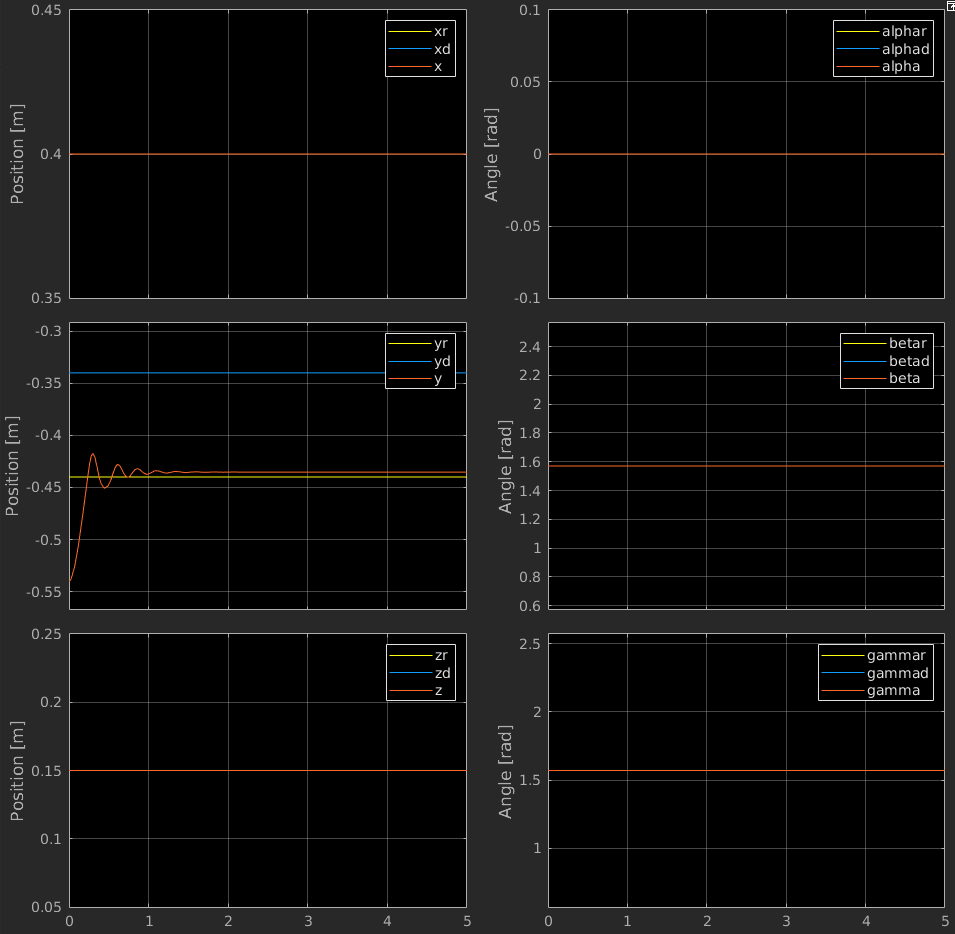
\includegraphics[keepaspectratio,width=\textwidth]{compliance_1000}
\caption{Compliance control - $K=1000$}
\end{figure}

\newpage

\section{Assignment 12}

\subsection{Implement the impedance control in the operational space}

\begin{figure}[H]
\centering
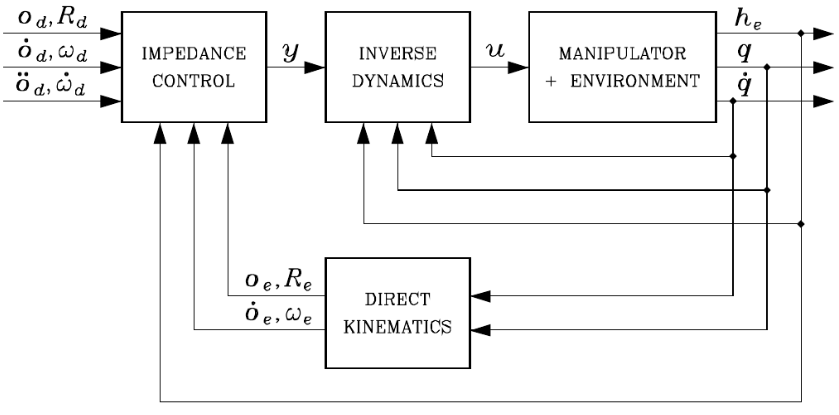
\includegraphics[keepaspectratio,width=.5\textwidth]{impedance_arch}
\caption{Impedance control in operational space architecture}
\end{figure}

The architecture implements the following stabilizing linear control law:

\begin{equation*}
y = J_A^{-1}(q)M_d^{-1}(K_D\dot{\tilde x} + K_P\tilde x - M_d\dot J_A(q,\dot q)\dot q - M_db(\tilde x,R_d,\dot o_d,\omega_d)-h_e^d)
\end{equation*}

The architecture is based on the definition of a mechanical impedance defined by an equivalent mass matrix $M_d$, an equivalent damping matrix $K_D$ and an equivalent stiffness matrix $K_P$. The mechanical impedance is independent from the configuration of the robot.

The architecture is modelled in SIMULINK as follows:

\begin{figure}[H]
\centering
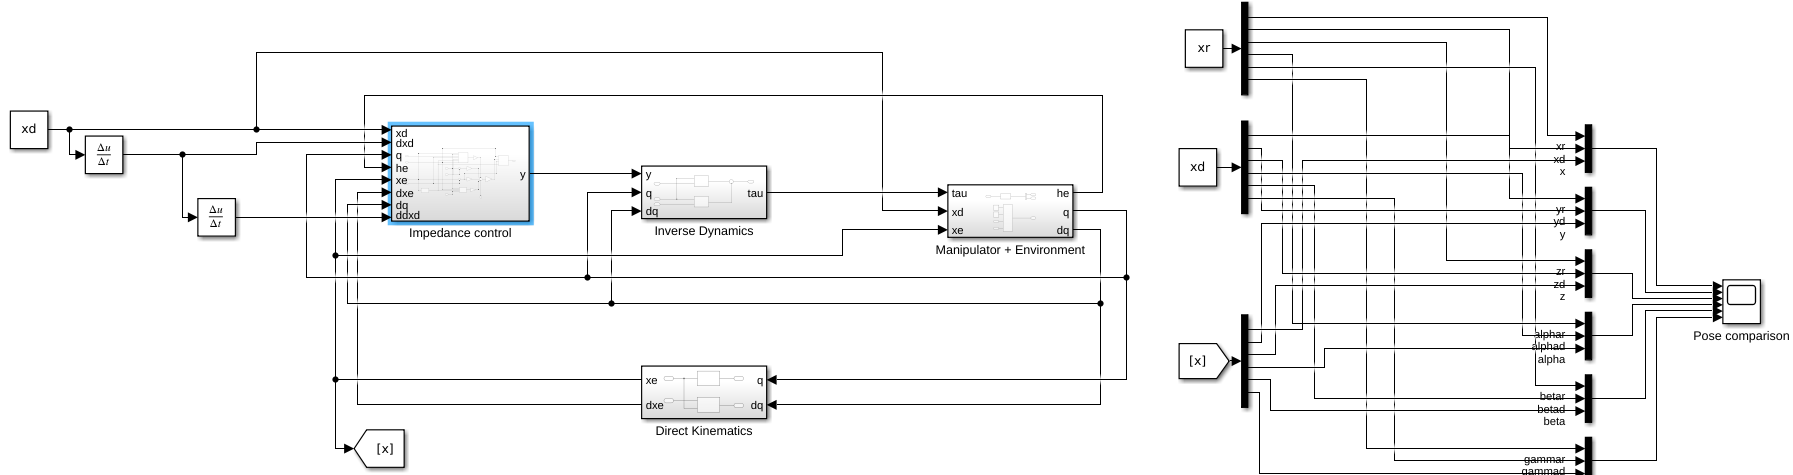
\includegraphics[keepaspectratio,width=\textwidth]{impedance_sim}
\caption{Impedance control in operational space SIMULINK model}
\end{figure}

To test the architecture, the manipulator was moved to $x_0=k(\begin{bmatrix}
0&-0.3&0
\end{bmatrix})$, with a desired position of $x_d=k(\begin{bmatrix}
0&-0.2&0
\end{bmatrix})$ and the environment placed at $x_e=k(\begin{bmatrix}
0&-0.1&0
\end{bmatrix})$. This was done to simplify the architecture, allowing for contact only in the $y$ direction. The mechanical impedance was defined with $M_d=\begin{bmatrix}
0.3 & 1 & 0.3 & 0.3 & 0.3 & 0.3
\end{bmatrix}$, $K_D=\begin{bmatrix}
30 & 25 & 30 & 30 & 30 & 30
\end{bmatrix}$ and $K_P=\begin{bmatrix}
50 & 75 & 50 & 50 & 50 & 50
\end{bmatrix}$.

\newpage

\begin{figure}[H]
\centering
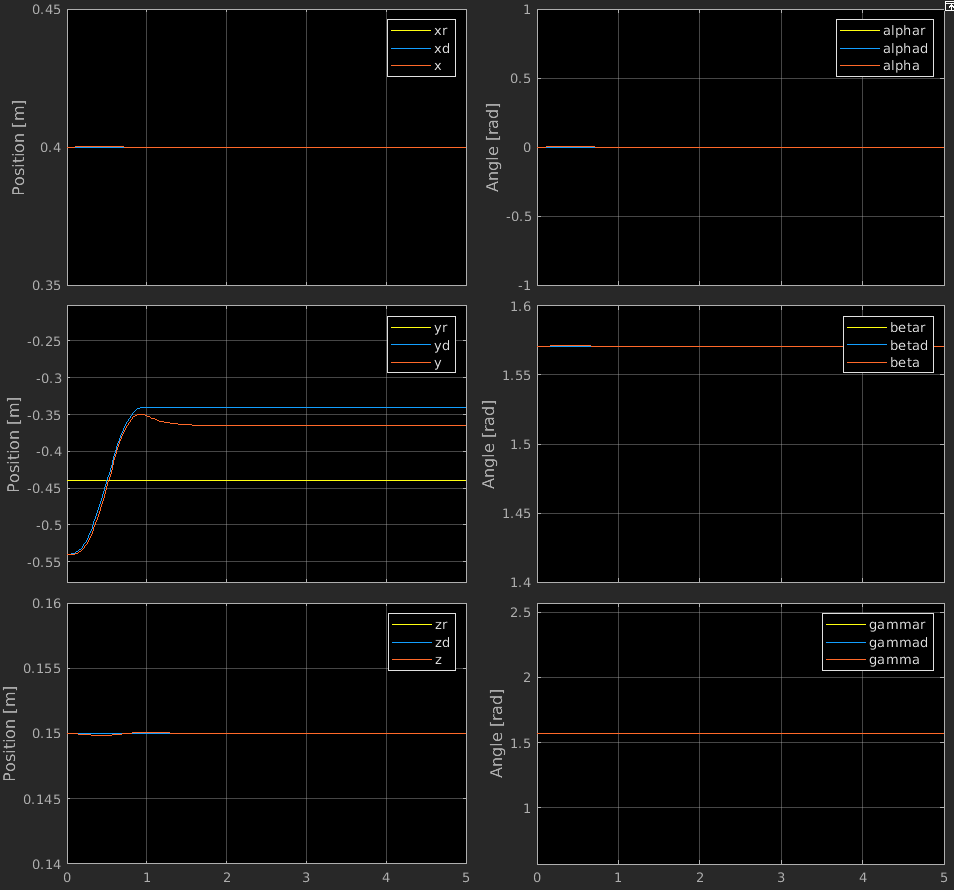
\includegraphics[keepaspectratio,width=\textwidth]{impedance_1}
\caption{Impedance control}
\end{figure}

\newpage

\section{Assignment 13}

\subsection{Implement the admittance control in the operational space}

\begin{figure}[H]
\centering
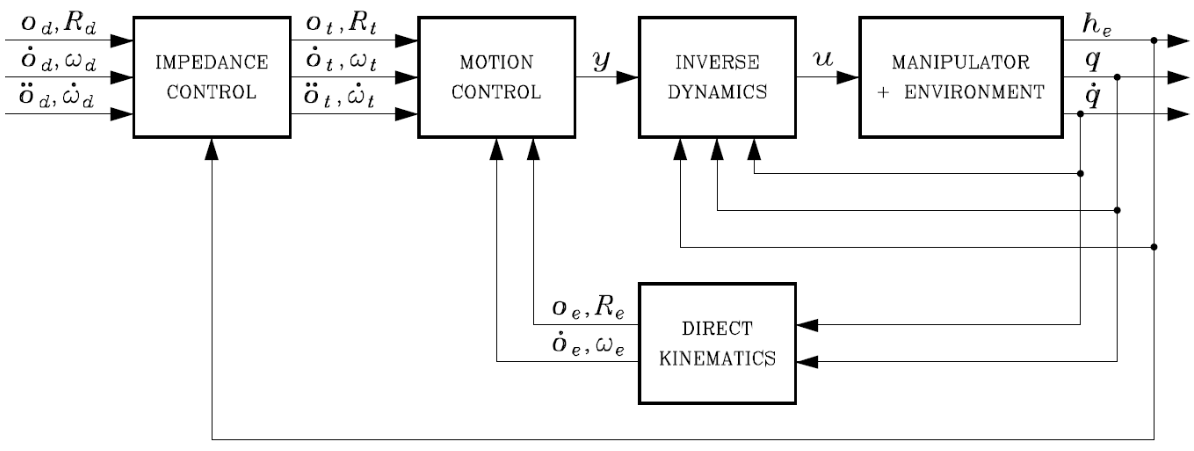
\includegraphics[keepaspectratio,width=.5\textwidth]{admittance_arch}
\caption{Admittance control in operational space architecture}
\end{figure}

The relationship between the external interaction force $h_e^d$ and the operational space error $\tilde z$ is defined through an admittance:

\begin{equation*}
M_t\ddot{\tilde z}+K_D\dot{\tilde z}+K_P\tilde z = h_e^d
\end{equation*}

The operational space error is between the desired frame and a compliant frame, introduce to force a compliant behaviour of the end-effector. The manipulator then always follows the compliant trajectory, which is equal to the desired one only in absence of external disturbances.

The architecture is modelled in SIMULINK as follows:

\begin{figure}[H]
\centering
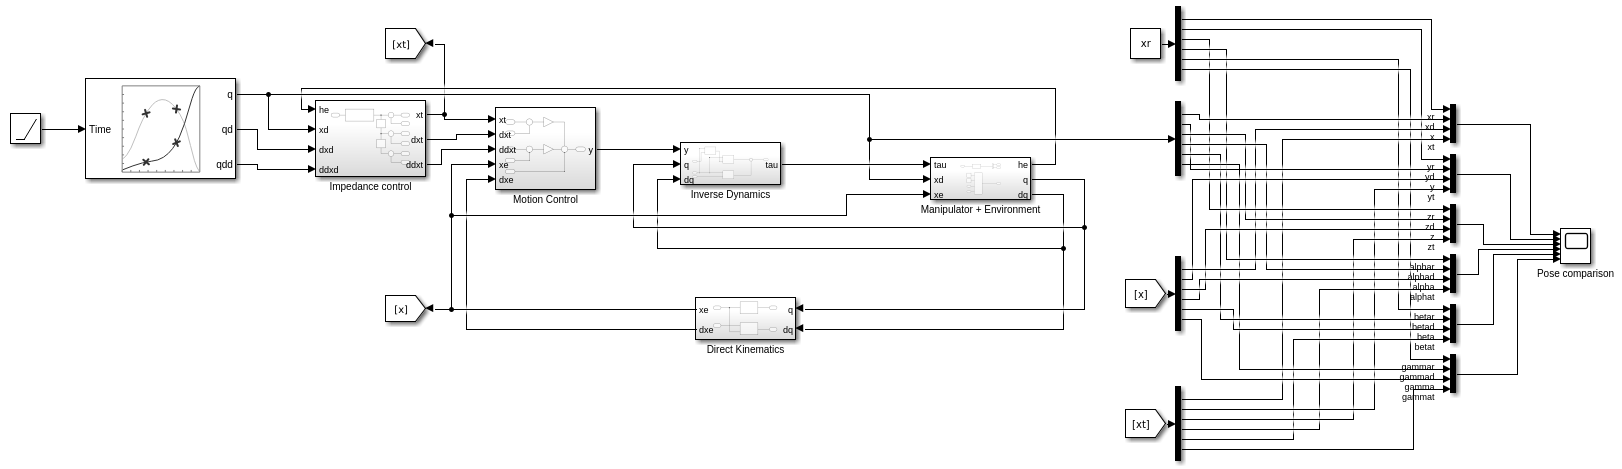
\includegraphics[keepaspectratio,width=\textwidth]{admittance_sim}
\caption{Admittance control in operational space SIMULINK model}
\end{figure}

To test the architecture, the manipulator was moved to $x_0=k(\begin{bmatrix}
0&-0.3&0
\end{bmatrix})$, with a desired position of $x_d=k(\begin{bmatrix}
0&-0.25&0
\end{bmatrix})$ and the environment placed at $x_e=k(\begin{bmatrix}
0&-0.2&0
\end{bmatrix})$. This was done to simplify the architecture, allowing for contact only in the $y$ direction. The mechanical impedance was defined with $M_t=\begin{bmatrix}
1 & 1 & 1 & 1 & 1 & 1
\end{bmatrix}$, $K_{Dt}=\begin{bmatrix}
1 & 10 & 1 & 1 & 1 & 1
\end{bmatrix}$ and $K_{Pt}=\begin{bmatrix}
1 & 20 & 1 & 1 & 1 & 1
\end{bmatrix}$ , while the control law is defined by $K_D=\begin{bmatrix}
10 & 10 & 10 & 10 & 10 & 10
\end{bmatrix}$ and $K_P=\begin{bmatrix}
50 & 50 & 50 & 50 & 50 & 50
\end{bmatrix}$.


\newpage

\begin{figure}[H]
\centering
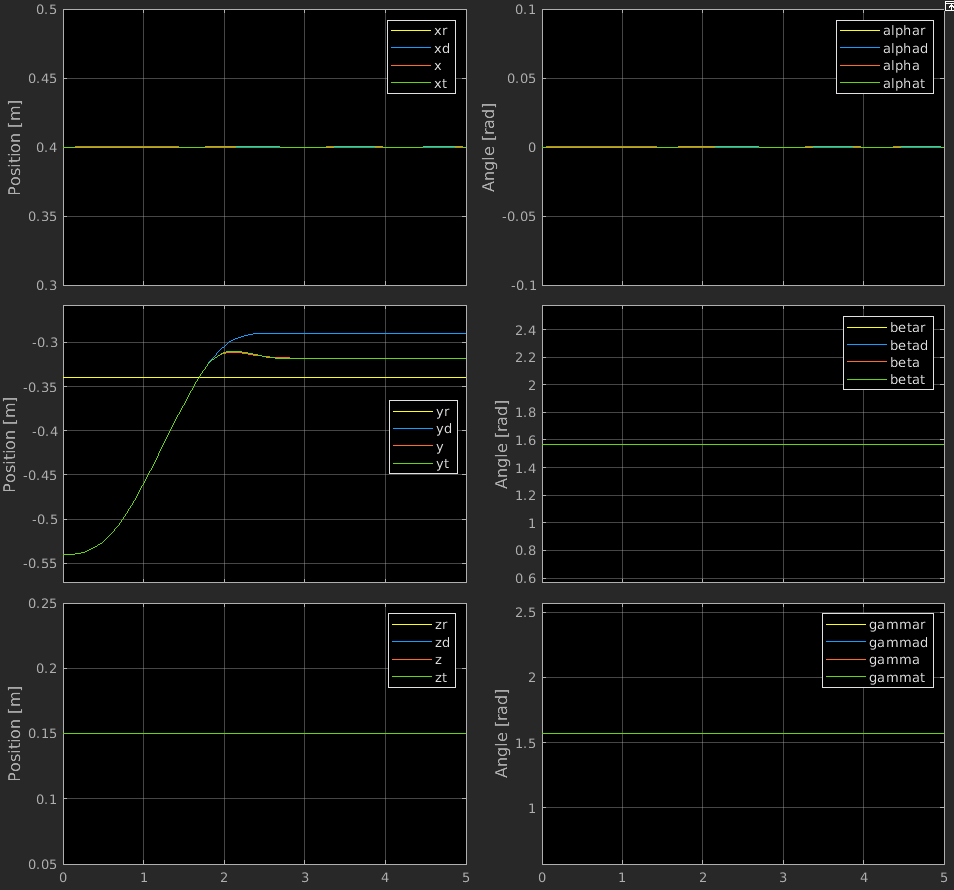
\includegraphics[keepaspectratio,width=\textwidth]{admittance_1}
\caption{Admittance control}
\end{figure}

\newpage

\section{Assignment 14}

\subsection{Implement the force control with inner position loop}

\begin{figure}[h]
\centering
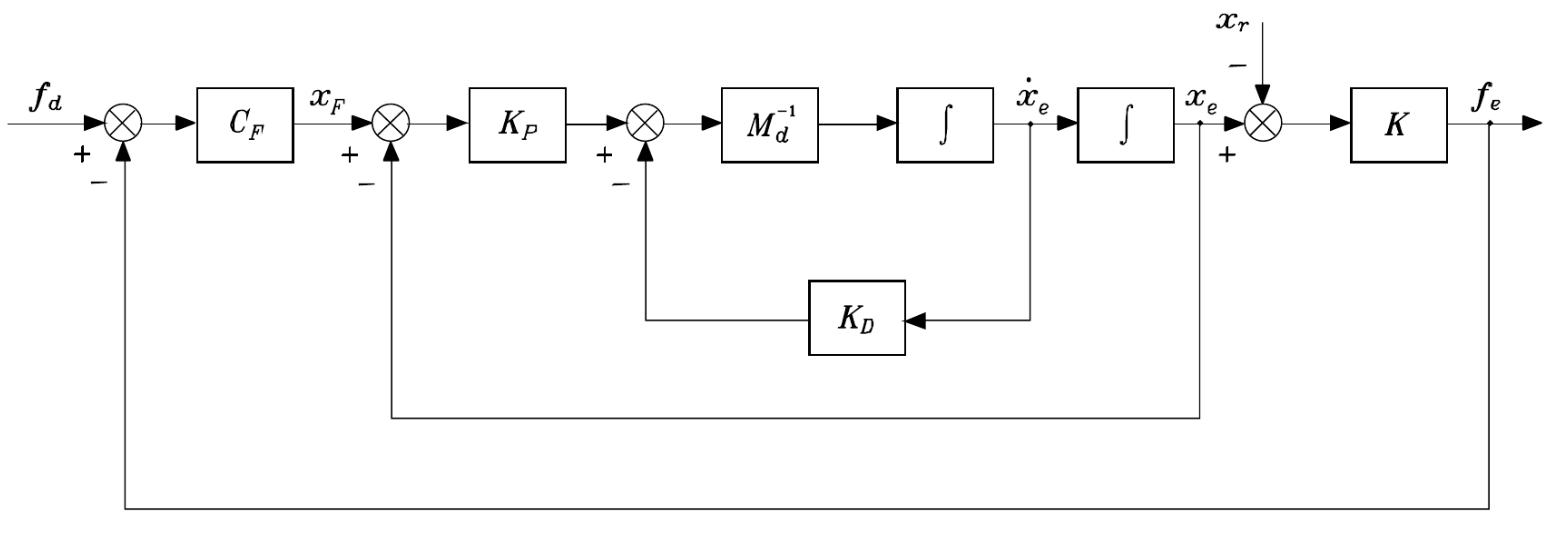
\includegraphics[keepaspectratio,width=0.8\textwidth]{force_arch}
\caption{Force control with inner position loop architecture.}
\end{figure}

The architecture is based on an inverse dynamic position control surrounded by a force feedback loop. Given a desired constant force reference $f_d$ we define a diagonal matrix $C_F$ that acts like a compliant matrix, mapping force into position:

\begin{equation*}
x_F = C_F(f_d-f_e)
\end{equation*}

where $f_e$ is the measured interaction force.

The shape of the controller $C_F$ is important. If $C_F$ is a PI controller, i.e. $C_F=K_F+\frac{1}{s}K_I$, then the steady state error is null.

The architecture is modelled in SIMULINK as follows:

\begin{figure}[h]
\centering
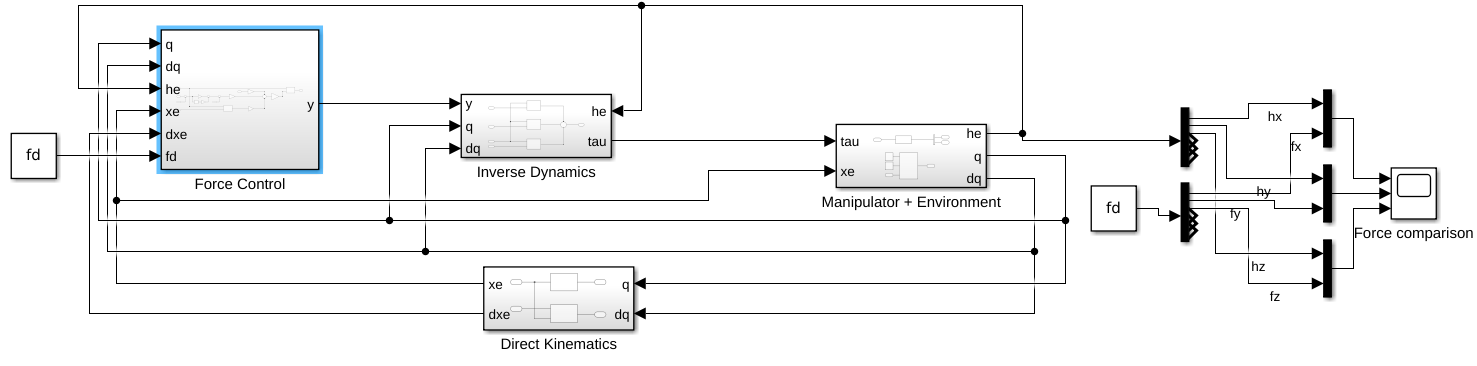
\includegraphics[keepaspectratio,width=0.8\textwidth]{force_sim}
\caption{Force control with inner position loop SIMULINK model.}
\end{figure}

The architecture was tested with $f_d = \begin{bmatrix}
0 & 1 & 0 & 0 & 0 & 0
\end{bmatrix}$, with an environment stiffness $K=5\mathbb I_6$, PI gains for the force loop $K_I=5\mathbb I_6$ and $K_F=10\mathbb I_6$.

\begin{figure}[h]
\centering
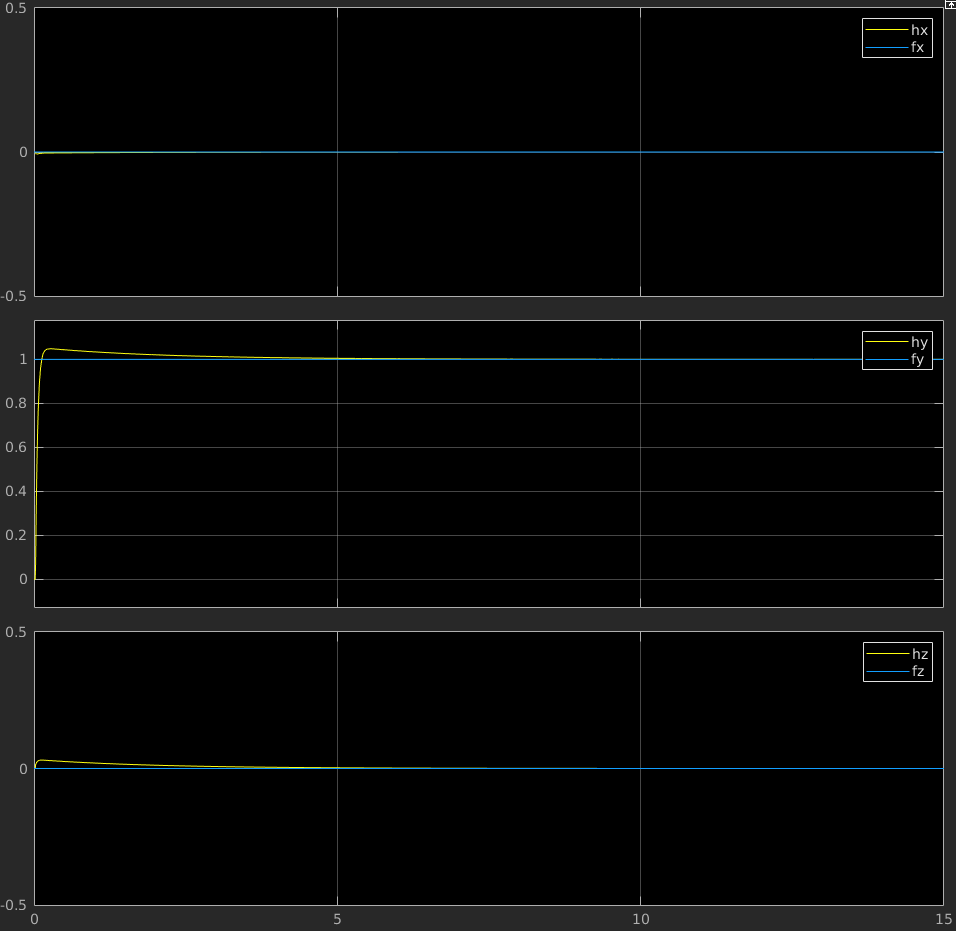
\includegraphics[keepaspectratio,width=0.6\textwidth]{force_1}
\caption{Force control with inner position loop - $C_F=K_F+\frac{1}{s}K_I$}
\end{figure}

\begin{figure}[h]
\centering
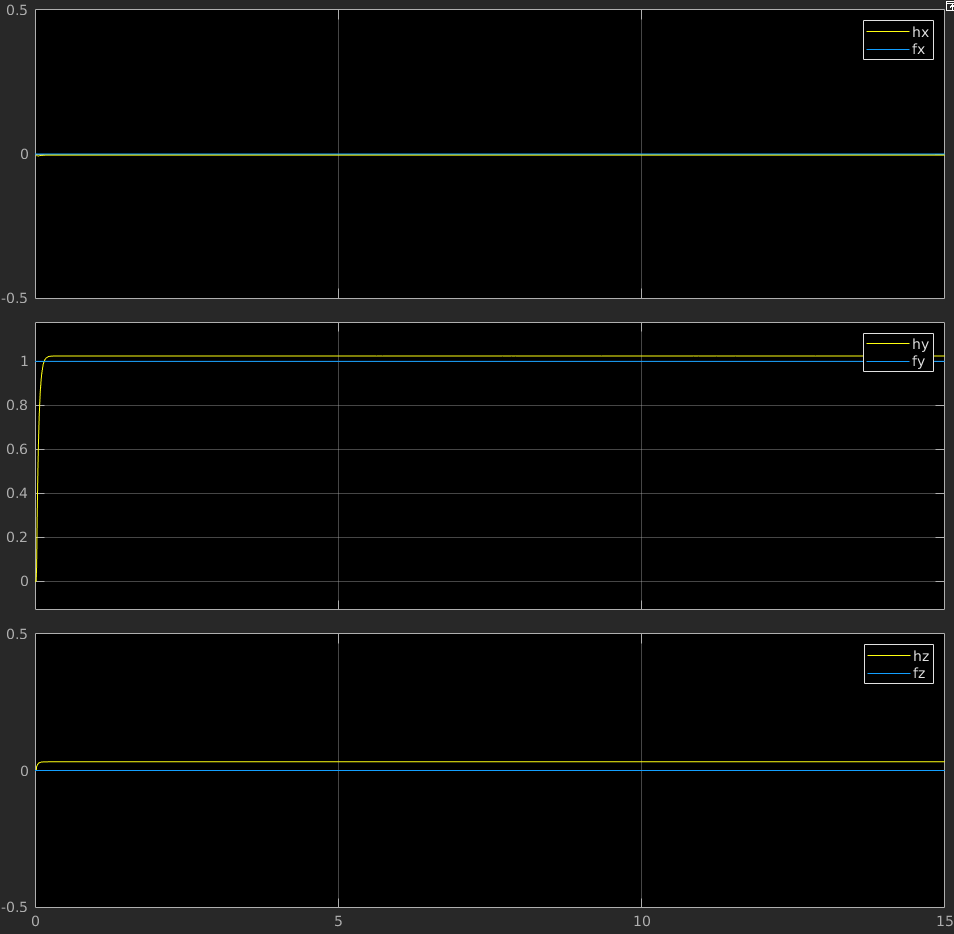
\includegraphics[keepaspectratio,width=0.6\textwidth]{force_noi}
\caption{Force control with inner position loop - $C_F=K_F$}
\end{figure}

\newpage

\section{Assignment 15}

\subsection{Implement the parallel force/position control}

\begin{figure}[h]
\centering
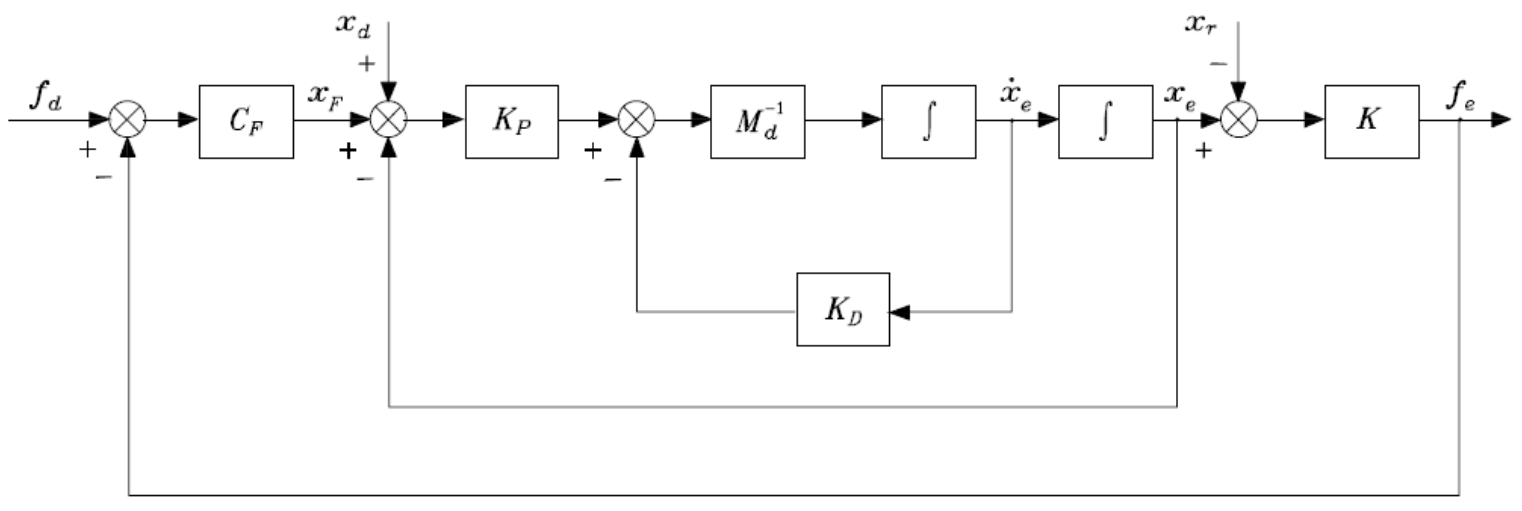
\includegraphics[keepaspectratio,width=0.8\textwidth]{parallel_arch}
\caption{Parallel force/position control architectures.}
\end{figure}

The architecture is essentially the same as the force control with inner position loop. The main difference is that we actually introduce the desired end-effector pose $x_d$ into  the position loop.

The architecture is implemented in SIMULINK as follows:

\begin{figure}[h]
\centering
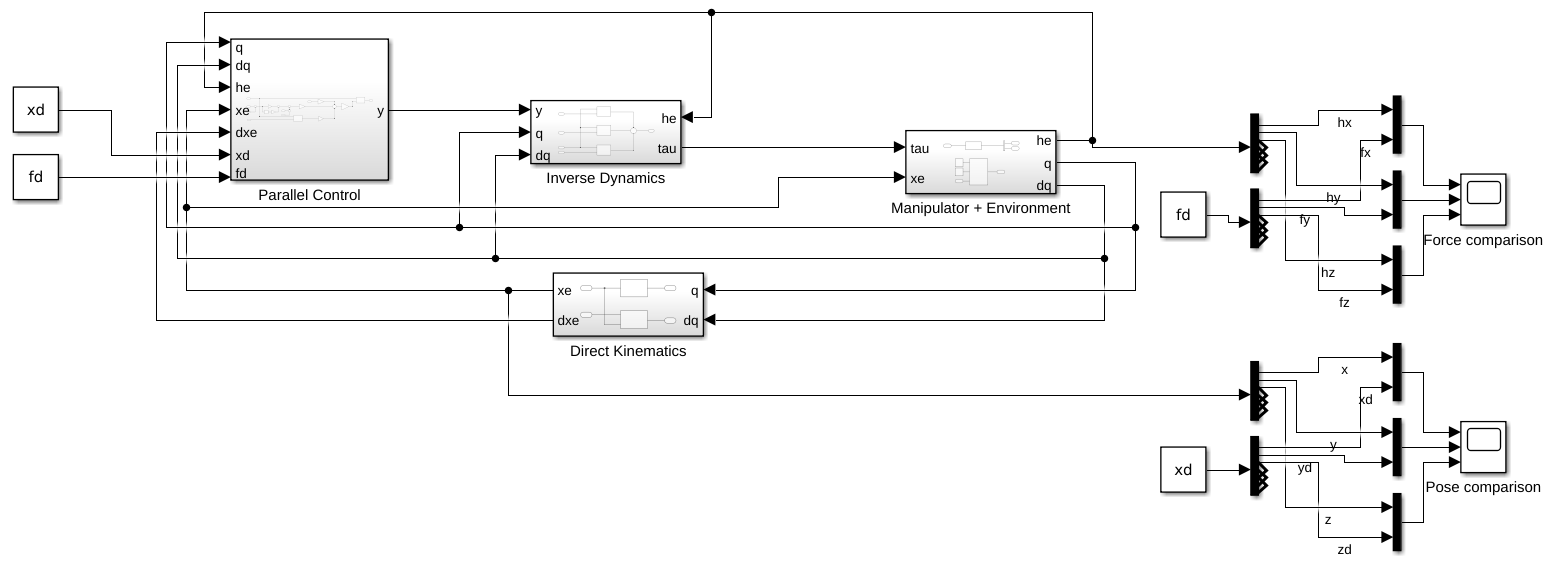
\includegraphics[keepaspectratio,width=0.8\textwidth]{parallel_sim}
\caption{Parallel force/position control SIMULINK model.}
\end{figure}

\newpage

The architecture was tested with $f_d = \begin{bmatrix}
0.5 & 0 & 0 & 0 & 0 & 0
\end{bmatrix}$, with an environment stiffness $K=\begin{bmatrix}
1 & 0 & 0 & 0 & 0 & 0
\end{bmatrix}$, PI gains for the force loop $K_I=15\mathbb I_6$ and $K_F=15\mathbb I_6$. The desired pose is $k(\begin{bmatrix}
-\pi/2 & -0.1 & -\pi/6
\end{bmatrix})$ while the environment is placed at  $k(\begin{bmatrix}
-\pi/2 & -0.2 & -\pi/6
\end{bmatrix})$.

\begin{figure}[h]
\centering
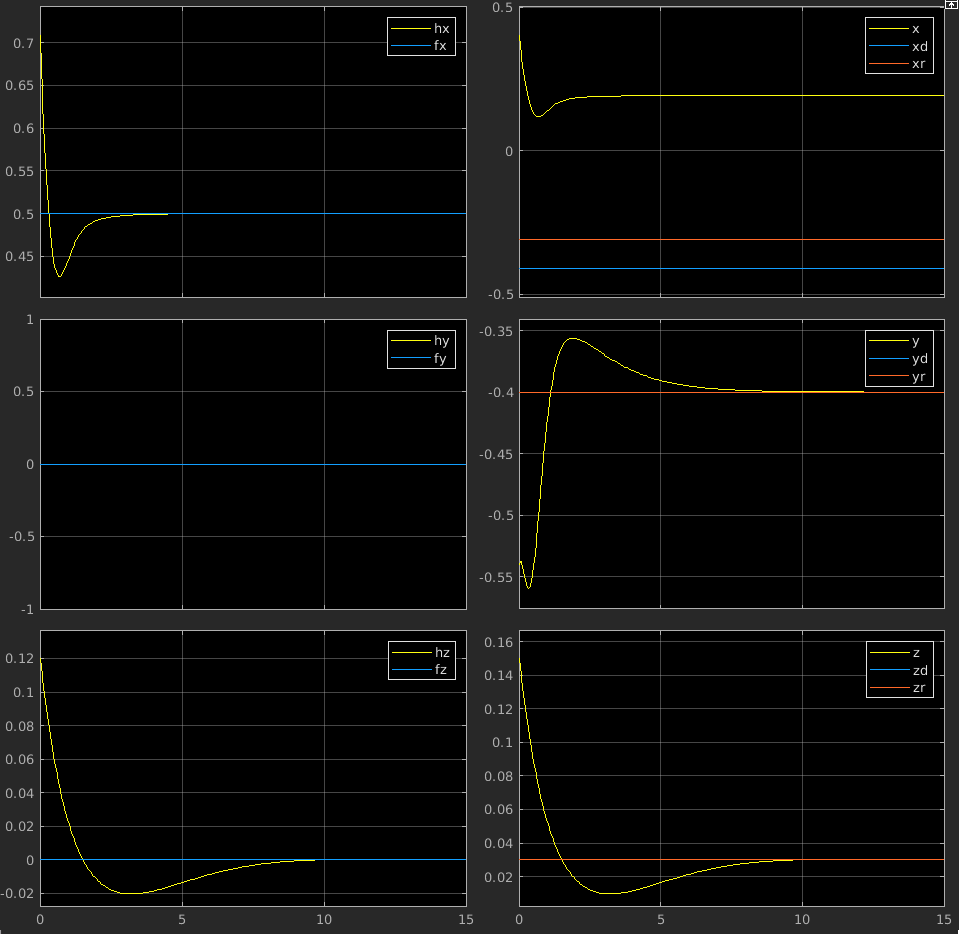
\includegraphics[keepaspectratio,width=0.8\textwidth]{parallel}
\caption{Parallel force/position control}
\end{figure}


\end{document}
